\documentclass[preprint, doubleblind, authoryear,10pt]{elsarticle}
% \documentclass[doubleblind, authoryear,10pt]{elsarticle}
% \documentclass[review, authoryear,12pt]{elsarticle}
% \documentclass[12pt, a4paper, oneside, article]{article}
\journal{TBD}

\usepackage[margin=2cm]{geometry}
\usepackage{a4wide}
\usepackage{fullpage}

\usepackage[english]{babel}
%\usepackage[latin1]{inputenc}
\usepackage[utf8]{inputenc}
\usepackage[T1]{fontenc}
%\usepackage[ansinew]{inputenc}

\usepackage{amsmath, amsfonts, amssymb}

\usepackage{lscape}
\usepackage{graphicx} 
\usepackage{graphics}
\usepackage{subfig}
\usepackage{ae}
\usepackage{pdflscape}
\usepackage{setspace}
\usepackage{tabularx}
\usepackage{dcolumn}
\usepackage{rotating}
\usepackage{supertabular}
\usepackage{multirow}
\usepackage{longtable}
\usepackage[flushleft]{threeparttable}
\usepackage{rotating}
\usepackage{color}
\usepackage{xcolor}
\usepackage{bm}
% \usepackage{tcolorbox}
\usepackage{hyperref} % referencias dentro do texo (*QUEBRA MEMOIR*)
\hypersetup{colorlinks=true, citecolor=blue, urlcolor=blue, linkcolor=red,}
\usepackage{url}

%%%%%%%%%%%%%%%%%%%%%%%%%%%%%%%%%%%%%%%%%%%%%%%%%%%%%%%%%%%%%%%%%%%%%%%%%%%%%%%%%%%%%%%%%%%%%%%
%%%%%%%%%%%%%%%%%%%%%%%%%%%%%%%%%%%%%%%%%%%%%%%%%%%%%%%%%%%%%%%%%%%%%%%%%%%%%%%%%%%%%%%%%%%%%%%
\begin{document}

%%%%%%%%%%%%%%%%%%%%%%%%%%%%%%%%%%%%%%%%%%%%%%%%%%%%%%%%%%%%%%%%%%%%%%%%%%%%%%%%%%%%%%%%%%%%%%%
% frontmatter

\begin{frontmatter}

\title{Index Tracking with Feature Selection}%\footnote{}

\author[Label1]{Paulo Ferreira Naibert\fnref{label1}}
\author[Label2]{Jo\~ao F. Caldeira}
\fntext[label2]{Corresponding author. Department of Economics, Universidade Federal do Rio Grande do Sul, Porto Alegre, R.S. 90040-000, Brazil. Telephone: +55-51. Fax: +55-51. e-mail: paulo.naibert@gmail.com}
%%
\address[Label1]{PhD Candidate at the Economics Department of the Federal University of Rio Grande do Sul}
\address[Label2]{Department of Economics, Universidade Federal de Santa Catarina}

% \begin{singlespace}
\begin{abstract}
\noindent
We compare the performance of passive investment portfolio with a small number of assets (sparse index-tracking portfolios) using different feature selection algorithms.
To isolate the effect of the selection methods, we separate the asset selection and the asset allocation phase.
In the asset allocation phase, we follow \cite{liu-2009}, and select minimum tracking error volatility portfolios.
The selection methods used are the backward stepwise selection, forward stepwise selection and the lasso.
\textbf{RESULTS}
\end{abstract}
% \begin{singlespace}

%\noindent\textit{JEL classification:} C53; E43; G17.\\
%\noindent\textit{Keywords:} portfolio optimization, yield curve forecasts, bond indexing, Kalman filter, out-of-sample evaluation.

\begin{keyword}
Index-Tracking; \sep Portfolio Theory; \sep Feature Selection; \sep Optimal Portfolios 

\noindent\textit{JEL classification:} G11; G12; G17.
\end{keyword}

\end{frontmatter}

%%%%%%%%%%%%%%%%%%%%%%%%%%%%%%%%%%%%%%%%%%%%%%%%%%%%%%%%%%%%%%%%%%%%%%%%%%%%%%%%%%%%%%%%%%%%%%%
% text 
\clearpage

%%%%%%%%%%%%%%%%%%%%%%%%%%%%%%%%%%%%%%%%%%%%%%%%%%%%%%%%%%%%%%%%%%%%%%%%%%%%%%
% intro
\section{Introduction} \label{sec:intro}

% -------------------------------------
% \subsection*{Research Territory}

\cite{tz2011} and \cite{liu-2009} point out that the majority of institutional investors are benchmarked by an index, e.g. the SP500.
So, their performance has to be evaluated in relation to that index.
Consequently, having to choose index tracking portfolio is closer to the practical life of a institutional investor.
Index tracking can be defined as a quantitative method of trading and of passive portfolio management \citep{PLS10, nnl14}.
The most popular way to use this strategy is to form a portfolio of assets to mimic the performance of an externally specified index that, usually, is a market index such as the SP500.
This performance takes into account the risk-return profile of the specified benchmark.

% two main ways
There are two main ways of maintaining a fund that tracks an index; one is the full replication and the other is the partial replication.
% full replication
Full replication is the simplest one; it consists on maintaining all the assets with the same relative weights of the index being tracked.
However, despite being possible to achieve a perfect replication with it, the full replication presents some disadvantages:
(i) it results in small weights, which increase transaction costs;
(ii) it presents instability of the weights, which means frequent revisions of them;
(iii) its portfolio rebalancing can become complicated; 
and (iv) price fluctuation bring too many additions and subtractions of assets to the index.

% partial replication
It is also possible to try to replicate an index with a portfolio that contains only a small proportion of all the available assets, this is the partial replication.
But this method also presents some problems:
(i) the initial selection of the small number of assets to be included in the portfolio can be hard, and
(ii) the need to estimate optimal weights (allocation) complicate the problem.

To implement an index tracking strategy, the investor has to solve two interconnected problems associated with it.
The first is the asset selection problem, where the investor selects $p$ assets from a universe of $N$ assets.
The second is the asset allocation problem, where the investor decides the relative weights of each selected asset.

% -------------------------------------
% \subsection*{What we do}
% minimize the tracking error volatility

The main goal of this paper is to compare the performance of different feature selection algorithms applied to index tracking and portfolio optimization.
More specifically, we study the case where an investor has to track an Index and he rebalances his portfolio monthly, bimonthly and quarterly (20, 40, and 60 days rebalancing).
First, we select the assets with the following strategies:
backward iteration, forward iteration, lasso regression.
Here, we highlight the use of the backward and forward iteration algorithms that receive very little attention in the literature.
With the selected assets, we form portfolios by minimizing the tracking error volatility.
Then, we take the out of sample portfolio returns and analyze those returns in comparison to the selected Index.
We use two differente datasets.
The first is a brazilian dataset of asset prices with daily frequency from January 1999 to December 2010 (2970 days).
The second is an american dataset of asset prices with daily frequency from January 2010 to October 2017 (1950 days).

The benefits of this two phase method is twofold.
First, it isolates the effect of the selection methods, so the differences in performance may be attributed to differences in asset selection methods.
Second, we make use of the Global Minimum Variance Portfolio (GMVP) in the second phase.
The GMVP has several desirable properties discussed in \cite{jag-2003} and \cite{CTS2006}.
As the goal of this paper is to compare the performance of the selection algorithms applied to index tracking and portfolio selection, this separation of phases is very suitable to our needs.

% -------------------------------------
% \subsection*{Lit Review}

Next, we list papers that evaluated different methods of asset selection and portfolio optimization to implement index tracking and we compare their works to ours.
%
\cite{liu-2009} selects portfolios that track the SP500 by minimizing tracking error volatility without regard for the size of mean of the tracking error.
In that paper, the asset selection phase is solved by only using the 30 assets in the Dow Jones Industrail Average (DJIA).
\cite{dijk2002} use index tracking with small portfolios by asset selection methods.
\cite{PLS10} mention the possibility that the problems of asset selection and portfolio optimization can be put in the form of variable selection.
They implement the asset selection with methods of penalized regression.
Thus, we can use other methods of variable selection to choose the assets that will enter our portfolio.
Here, we will use some methods listed in \cite{isl-2014}.

\cite{santos15} selects minimum variance portfolios using cardinality constraints to form portfolios with few assets and assess their performance.
\cite{rbfin-it} selects Index-Tracking portfolios with cardinality constraints to form portfolios with few assets and track the Bovespa Index.
This paper resembles those once we will form portfolios with few assets; however we will use a different method.
We will not use cardinality constraints, but feature selection algorithms.
This can be justified by the lower computational cost of those algorithms.
We will use only regressions to select the portfolio assets, the optimization of portfolios weights will occur in a different phase.

Other related works are \cite{nnl14} e \cite{nnen14}, which use non-negative lasso and elastic net regressions to select assets.
Those works use non-negative least-squares for portfolio optimization (weight selection).
Yet another related work is \cite{lasso-infl}, which use lasso regression to select variables to forecast inflation.
This work differs from that in terms of the goal for which we use the lasso regression.
Here we use it to form portfolios to track a financial Index.


% -------------------------------------
% \subsection*{Results prelim}
Our results show that, in the brazilian case, the lasso selection method outperforms the other methods by presenting similar tracking error volatility and higher mean returns.
Note that this overperformance is due only to asset selection, not due to the shrinkage of the portfolio weights that results from the consstraints of the problem.
This happens because the asset allocation is the same for all portfolios.
More on the shrinkage of portfolio weights can be found in \cite{fan-2012, jag-2003, brodie2009}.

However, in the american case, the lasso method presents more volatility, but this is more than offset by its superior mean returns, which ultimately delievers better risk-adjusted performance.
But, because our primary goal is to minimize tracking error volatility, this kind of risk-return tradeoff is not desirable in our case.
Even though the backward and forward selection methods might be outperformed by the lasso, there are some instances where these methods are superior or comparable to the benchmark index. 
This has to be highlighted, because those simple methods of feature selection receive too little attention in the portfolio literature, even though they might bring good results.

% -------------------------------------
% \subsection*{TOC}

Beyond this introduction, this paper is organized as follows.
Section \ref{sec:defs} presents the basics of portfolio selection that will be used throughout the paper.
Section \ref{sec:selection} presents the algorithms used to apply feature selection in the dataset.
Section \ref{sec:experiment} presents the methodology of the empirical study.
Section \ref{sec:results} shows the results obtained in the empirical study.
% Section \ref{sec:data} presents the data that will be used in this work.
Finally, the section \ref{sec:conc} concludes.

%%%%%%%%%%%%%%%%%%%%%%%%%%%%%%%%%%%%%%%%%%%%%%%%%%%%%%%%%%%%%%%%%%%%%%%%%%%%%%%%%%%%
% \clearpage
\section{Basic Definitions} \label{sec:defs}

In this section, we present the basics of portfolio selection that we will use throughout this paper.
We start by considering an investment universe with $N$ risky assets.
Each asset has a price in time $t$ denoted by $P_{t,i}$.
By holding asset $i$ from $t-1$ to $t$, the investor earns the return
\begin{align} \label{eq:ret}
	X_{t,i} = \frac{P_{t,i}}{P_{t-1,i}} - 1.
\end{align}

Let's  denote the $N\times1$ vector of future and uncertain returns of those assets in time $t$ by $X_{t}$, where 
\begin{align*} % \label{ret_vec}
	X_{t} =  [X_{t1}, X_{t2} , \dots, X_{tN}]'.
\end{align*}
We will assume that the returns have mean vector $E[X_{t}] =\mu_{X}$ and covariance matrix $V[X_{t}] =\Sigma$.
We also denote the future and uncertain return of the index by $y_{t}$.
We assume that the index return have mean $E[y_{t}] = \mu_{y}$ and variance $V[y_{t}]=\sigma^2_{y}$.


% excess returns
With those definitions, we can define the \textbf{excess returns} of the risky assets on the index as:
\begin{align*}
	R_{t} &= X_{t} - e y_{t}.
\end{align*}
where $e$ is a $N \times 1$ vector of ones.
We assume that $R_{t}$ has mean vector and covariance matrix 
\begin{align*}
E[R_{t}] &= \mu_{X}-e\mu_{y}=\mu
\\
V[R_{t}] &= \Sigma + \sigma_{y}^{2}ee' - 2Cov(X_{t},y_{t})e' =\Omega.
\end{align*}


%%%%%%%%%%%%%%%%%%%%%%%%%%%%%%%%%%%%%%%%%%%%%%%%%%%%%%%%%%%%%%%%%%%%%%%%%%%%%%%%%%%%
% portfolio
\subsection*{Porfolio Returns}

Next, we define portfolio and portfolio returns.
A portfolio of the $N$ risky assets is represented by a $N\times 1$ vector $w$, where
\begin{align*}
	w = \left[ w_1, w_2 , \dots, w_N \right]',
\end{align*}
and $w_{i}$ is the fraction of total wealth invested in asset $i$.
The vector $w$ can also be called the allocation vector.
If we constrain the weights in $w$ to sum up to one ($e'w=1$), we have the \textbf{fully bought condition}.

Holding the portfolio $w_{t}$ from $t$ to $t+1$ yields the out-of-sample return in $t+1$,
\begin{align} \label{eq:retport}
	X_{p,t+1} &= w_{t}'X_{t+1}.
\end{align}
$X_{p,t+1}$ is a weighted average of the asset returns selected to the portfolio with weights $w_{i}$ for $i=1,\dots,N$.
\begin{align*} \label{ret_port}
	X_{p,t+1} = w_{t,1} X_{t+1,1} + \dots + w_{t,N} X_{t+1,N}
	= \sum_{i=1}^{N} w_{t,i} X_{t+1,i} = w_{t}'X_{t+1}.
\end{align*}

%%%%%%%%%%%%%%%%%%%%%%%%%%%%%%%%%%%%%%%%%%%%%%%%%%%%%%%%%%%%%%%%%%%%%%%%%%%%%%%%%%%%
% Evolution of Weights
\subsection*{Evolution of weights}

\cite{liu-2009} points out that in the moment prior to rebalancing, each dollar invested in asset $i$ in the portfolio has changed its value from $w_{t,i}$ to $w_{t,i}(1+X_{t+1,i})$, where $w_{t,i}$ is the $i$-th element of $w_{t}$ and the $i$-th element of $X_{t}$ is denoted as $X_{t,i}$.
Also, in general, each dollar invested in the whole portfolio has changed from $w_{t}$ to $w_{t}(1+X_{p,t+1})$.
Therefore, prior to rebalancing, the weight on asset $i$ has changed from $w_{i,t}$ to 
\begin{align*}
	w_{t,i}^{+1} &= w_{t,i} \dfrac{1+X_{t+1,i}}{1+w_{t}'X_{p,t+1}}.
\end{align*}

More generally, we can express equation the changed vector of weights as
\begin{align}
	\label{eq:wplus1}
	w_{t}^{+1} &= w_{t} \odot \frac{e + X_{t+1}}{1 + X_{p,t+1}},
\end{align}
where $\odot$ denotes the Hadamard (direct) product.
Compounding another period, the portfolio $w_{t}$ in $t+2$ will have changed to
\begin{align*}
	w_{t}^{+2} &= w_{t} \odot 
	\frac{(e + X_{t+1})\odot(e + X_{t+2})}{(1 + X_{p,t+1})\times(1 + X_{p,t+2})}.
\end{align*}

Following this logic, we reach a equation for $h$ periods:

\begin{align}
	\label{eq:wplush}
	w_{t}^{+h} &= w_{t} \odot 
	\frac{(e + X_{t+1})\odot\dots\odot(e + X_{t+h})}
	{(1 + X_{p,t+1})\times \dots \times(1 + X_{p,t+h})}.
\end{align}

%%%%%%%%%%%%%%%%%%%%%%%%%%%%%%%%%%%%%%%%%%%%%%%%%%%%%%%%%%%%%%%%%%%%%%%%%%%%%%%%%%%%
% Tracking Error
\subsection*{Tracking Error}

The tracking error may be defined as a measure of the difference between the index tracking portfolio return, $X_{p,t}$ and the index return, $y_{t}$.
So, we have the following expression for the tracking error:
\begin{align} 
	\label{eq:TE}
	TE_{t+1} &= w_{t}'X_{t+1} - y_{t+1} 
	= X_{p, t+1} - y_{t+1},
\end{align}
where $w_{t}$ is the allocation vector of our portfolio.

With the expression of the tracking error above, we can see that, if the weights are restricted to sum up to one ($e'w=1$), then the excess return of a portfolio on a benchmark is the same as the tracking error:
\begin{align}
	\notag
	R_{p,t+1} & = w_{t}'R_{t+1} = w'(X_{t+1} - e y_{t+1})
	\\
	\notag
	& = w_{t}'X_{t+1} - w'e y_{t+1}
	\\
	\label{eq:TER}
	R_{p,t+1} & = X_{p,t+1} - y_{t+1} = TE_{t+1}.
\end{align}
Hence, if the weights sum up to one ($e'w=1$), minimizing the variance of the Tracking Error is equivalent to minimizing the variance of the excess returns of a portfolio on a benchmark.
Note that the restriction is important.


%%%%%%%%%%%%%%%%%%%%%%%%%%%%%%%%%%%%%%%%%%%%%%%%%%%%%%%%%%%%%%%%%%%%%%%%%%%%%%%%%%%%
% \clearpage
\section{Feature Selection Algorithms} \label{sec:selection}

Here, we present the methods through which we will select the assets, they are:
(i) forward stepwise selection, 
(ii) backward stepwise selection, 
and
(iii) lasso regression,
More information about this methods can be found in \cite{isl-2014}.
The methods of asset selection used here depend heavily on the Ordinary Least Squares (OLS) Regression.
Below, we offer more details about these methods, beggining with some notes on the OLS Regression.

%%%%%%%%%%%%%%%%%%%%%%%%%%%%%%%%%%%%%%%%%%%%%%%%%%%%%%%%%%%%%%%%%%%%%%%%%%%%%%%%%%%%
% OLS
\subsection{Ordinary Least Squares (OLS) Regression}

By regressing the index returns against the asset returns with the portfolio weights being parameters to estimate, we have a regression problem with stochastic regressors, more details about this problem can be found in \cite{rao-2008} and \cite{rencher-2007}.
We may represent this problem as:
\begin{align*} 
	y_{t} &= \alpha + X_{t}\beta + \varepsilon_{t}.
\end{align*}
Note that the intercept $\alpha$ is necessary to let $E[\varepsilon_{t}]=0$, so we can have $V[\varepsilon_{t}] = E[\varepsilon_{t}^2]$.

The OLS regression has the goal to minimize the sum of squared residuals, which is expressed as:
\begin{align} \label{eq:rss}
	RSS(\beta)
	= \sum_{t=1}^{T} \varepsilon_t^2
	= \sum_{t=1}^{T} (y_t - \alpha - X_t \beta)^2.
\end{align}
where $\varepsilon_{t}$ is the residual of the regression.
% \begin{align*} 
% 	\varepsilon_{t} = y_{t} - \alpha -  X_{t} \beta.
% \end{align*}

By minimizing $RSS(\beta)$ in equation \eqref{eq:rss}, we find $\beta_{ols}$:
\begin{align} 
	\label{eq:bols}
	\beta_{ols} = (X'X)^{-1}(X'y)
\end{align}
where $X$ is the $J \times N$ matrix of asset returns: $X = [X_{t-J}, X_{t-J+1}, \dots , X_{t-1}]'$ and $y$ is the $J\times 1$ vector of index returns $y = [y_{t-J}, y_{t-J+1}, \dots , y_{t-1}]'$.

%=======================================================================
\subsection{Forward Stepwise Selection}

The forward stepwise selection uses a series of OLS regressions to select the assets that will enter the investor's portfolio, i.e. the columns that will enter in the matrix $X$.
It starts with a null model with no predictor, then we add one predictor at a time to the model until all predictors are added to the model.
More specifically, at each step the variable that provides the best fit is added to the model.

%=======================================================================
\subsection{Backward Stepwise Selection}

In opposition to the forward stepwise selection, the backward stepwise selection starts with the full OLS model, which contains all $N$ predictors available, then the least useful predictors are removed, one at a time, until we reach a model with the desired $p$ predictors.

The forward and backward stepwise selections result in a set of models, each of which contains a subset of $p$ predictors.
Usually, the researcher determines which of the models in the set of models is the best.
Here, however, we want a predefined number of assets in our portfolios.
So we just choose the model with the predefined number $p$ of assets with the smaller $RSS$ and bigger $R^2$.
To implement both of those algorithms, we  use the \texttt{R} software with the \texttt{leaps} package.\footnote{More information about the leaps package can be found in \url{https://cran.r-project.org/web/packages/leaps/}}

%=======================================================================
\subsection{LASSO}

To fit the least squares regression, we estimate the values of $\alpha, \beta_1, \cdots, \beta_p$ that minimize the $RSS$, as in equation \eqref{eq:rss}.
The lasso regression has a similar form, with its coefficients minimizing the $RSS$ plus a penalty: 
\begin{align} \label{lasso-reg} %\tag{6.7} 
\sum_{t=1}^{T} 
\left( y_t - \alpha - \sum_{j=1}^{p} \beta_j x_{tj} \right)^2 +
\lambda \sum_{j=1}^{p} |\beta_{j}| =
	RSS + 
	\lambda \sum_{j=1}^{p} |\beta_{j}| .
\end{align}
that is, the lasso is a penalized regression.
In the equation above, $\lambda \geq 0$ controls the amount of regularization in the regression.
When $\lambda = 0$, we have the least squares regression.
The bigger the value of $\lambda$, the bigger the amount of regularization and tighter the variable selection will be.
Thus, we have to fit $\lambda$ in a convenient way to our objectives.
In this paper we use the \texttt{glmnet} package of the \texttt{R} software.\footnote{More information about the glmnet package can be found in \url{https://cran.r-project.org/web/packages/glmnet/}}

Because the betas in the algorithms above might not sum to one, we only use the algorithms to select the assets.
\cite{nnl14} and \cite{nnen14} also segregate the asset selection phase and the asset allocation phase by doing different regressions for each phase.
Another reason to do this is that by using the same equation for all the portfolios' allocation, we can isolate the effect of the asset selection strategies.

%%%%%%%%%%%%%%%%%%%%%%%%%%%%%%%%%%%%%%%%%%%%%%%%%%%%%%%%%%%%%%%%%%%%%%%%%%%%%%%%%%%%
% EXPERIMENT
% \clearpage
\section{The Experiment} \label{sec:experiment}

In this section, we present the methodology of our experiment.
The goal of such experiment is to evaluate the performance of the alternative asset selection techniques against each other and the benchmark index.
It is done in three steps.
The first step is the asset selection phase, which is done by using the algorithms from section \ref{sec:selection}.
The second step is asset allocation phase, where we form optimal portfolios in pseudo real time.
The third step is the out of sample performance evaluation of those portfolios against each other and the benchmark.

%%%%%%%%%%%%%%%%%%%%%%%%%%%%%%%%%%%%%%%%%%%%%%%%%%%%%%%%%%%%%%%%%
% DATA
\subsection{Data} \label{sec:data}

In this empirical analysis we have two different datasets.
The first is the Brazilian dataset, it consists of daily closing prices for 61 stocks traded in the Bovespa and a series of daily closing prices for the Bovespa Index (IBovespa).
The sample period used here is from January 1999 to December 2010 (2970 days).
% The asset prices were drawn from Bloomberg, and the IBovespa series was obtained from the Sistema Gerenciador de Séries Temporais from the Brazilian Central Bank.
The second dataset is the American dataset, it consists of daily closing prices for 462 stocks and a series of daily closing prices for the SP500 index.
The sample period used here is from January 2010 to October 2017 (1950 days).

From the price and index series, we take the simple daily raw return of each asset, according equation \eqref{eq:ret}.
That will leave us with a total of $N+1$ ($N$ stocks plus one index) series of raw returns, with length of $T$, each.
With the raw return series ($X_{t}$), we use the algorithms from Section \ref{sec:selection} to select which assets will enter in our portfolios (asset selection phase).

%%%%%%%%%%%%%%%%%%%%%%%%%%%%%%%%%%%%%%%%%%%%%%%%%%%%%%%%%%%%%%%%%%%%%%%%%%%%%%%%%%%%
% Allocation
\subsection*{Allocation}
After that, we enter the asset allocation phase.
To that end, we follow \cite{liu-2009} and select portfolios that minimize the volatility of the tracking error, without any regard for the size of the mean of the tracking error.
To achieve this, we find the portfolio that minimizes the variance of the excess returns on the benchmark with a fully bought contraint ($e'w=1$).
The answer to the problem is:

\begin{align} \label{eq:gmv}
\Aboxed{%
w_{t} = \frac{\hat{\Omega}_{t}^{-1}e}{e'\hat{\Omega}_{t}^{-1}e} }
\end{align}
where $e$ is a $N \times 1$ vector of ones and $\hat{\Omega}_{t}$ is the covariance matrix estimator of $\Omega$ using information untill time $t$.

One clarification has to be made here, what the formula \eqref{eq:gmv} finds is the portfolio with the least variance of excess returns, without any regard for the mean.
So, following the index exactly and zeroing the tracking error is not a concern, only minimizing the volatility of the tracking error.
Using the equation \eqref{eq:gmv} can be defended on the grounds that it is the global minimum variance portfolio (GMVP).
This portfolio achieves just what we want and it offers several desirable properties as presented by \cite{jag-2003} and \cite{CTS2006}.
If we wanted to zero the tracking error, we would have to optimize a different objective function and use different restrictions in our portfolio.
However, this portfolio would not have the properties of the GMVP highlighted above.

%%%%%%%%%%%%%%%%%%%%%%%%%%%%%%%%%%%%%%%%%%%%%%%%%%%%%%%%%%%%%%%%%
% Rolling Windows
\subsection*{Rolling Windows}

To estimate the $\hat{\Omega}_{t}$ we adopt a recursive estimation approach based on a \textit{rolling window time series of returns} $\{R_{j}\}_{j=t}^{t+J-1}$ with $t$ varying from $t=1$ to $t=T-J-1$.
For this experiment, we use window length equal to $J=250$ for the Brazilian dataset and $J=500$ for the American dataset, because the American dataset has more assets, and we need $J>N$ for the covariance matrix to be invertible.
Other way to see that is by stacking $J$ vectors of excess returns on top of each other and form the $J \times N$ matrix 

\begin{align*}
R =
\begin{bmatrix}
	R_{t-J}	\\ R_{t-J+1} \\ \dots \\ R_{t-1}
\end{bmatrix}
\end{align*}

With the rolling windows' scheme, we form the vector of expected means and the covariance matrices of excess returns with the formulas:
\begin{align}
	\hat{\mu}_{t} &= J^{-1}\sum_{j=t}^{t+J-1} R_{t},
	\\
	\hat{\Omega}_{t} &= (J-1)^{-1} \sum_{j=t}^{t+J-1}(R_{t} - \hat{\mu})(R_{t} - \hat{\mu})'.
\end{align}
This results in $T-J-1$ estimates of expected return vectors and covariance matrices.
Using them, we find the allocation vector using equation \eqref{eq:gmv}.
By the end of this process, we generate $T-J-1$ allocation vectors for each asset selection algorithm, in each dataset.
With the allocation vectors, we compute the \textit{out-of-sample portfolio returns} with equation \eqref{eq:retport}, which generates the time series $\{X_{p,t+1}\}_{t=J}^{T-1}$.
This time series is the subject of our analysis. 

%%%%%%%%%%%%%%%%%%%%%%%%%%%%%%%%%%%%%%%%%%%%%%%%%%%%%%%%%%%%%%%%%%%%%%%%%%%%%%%%%%%%
% Evaluation Measures 
\subsection{Evaluation Measures} % \label{sec:eval}

What we will evaluate are the out-of-sample portfolio returns in relation to the benchmark index.
Since the goal of index tracking portfolio is to closely follow the series of interest, our evaluation has to consider how our portfolio performs in relation to the benchmark.
Note that, as \cite{tz2011} and \cite{liu-2009} point out, the majority of institutional investors are benchmarked by an index, e.g. the SP500.
So, their performance has to be evaluated in relation to that index.
Consequently, having to choose index tracking portfolio is closer to the practical life of a institutional investor.

%%%%%%%%%%%%%%%%%%%%%%%%%%%%%%%%%%%%%%%%%%%%%%%%%%%%%%%%%%%%%%%%%%%%%%%%%%%%%%%%%%%%

The statistics that we want to evaluate are the Sharpe Ratio (SR), which is the mean of portfolio returns divided by the standard deviation of the portfolio returns; and the Information Ratio (IR), which is the mean of the tracking error divided by the standard deviation of the tracking error.

% mean tracking error ($\mu_{p}$) and the standard deviation of the tracking error ($\sigma_{p}$).
% They have the following formulas:
% \begin{align}
% 	\hat{\mu}_{p} &= (T-J)^{-1}\sum_{t=J}^{T}R_{pt},
% 	\\
% 	\hat{\sigma}_{p} &= \sqrt{ (T-J-1)^{-1}\sum_{t=J}^{T} (R_{pt} - \mu)^2 }.
% \end{align}

% %%%%%%%%%%%%%%%%%%%%%%%%%%%%%%%%%%%%%%%%%%%%%%%%%%%%%%%%%%%%%%%%%%%%%%%%%%%%%%%%%%%%
% % Betas
% \subsubsection*{Portfolio Correlation and Beta}
% 
% Other important statistics are the correlation ($\rho$) and beta ($\beta$) of the portfolios' return against the IBovespa.

%%%%%%%%%%%%%%%%%%%%%%%%%%%%%%%%%%%%%%%%%%%%%%%%%%%%%%%%%%%%%%%%%%%%%%%%%%%%%%%%%%%%
% Turnover
\subsubsection*{Transaction Costs}

To get a sense of the amount of trading required to implement each portfolio strategy, we compute the portfolio turnover and report its average through time.
Turnover in time $t$ has the following formula
\begin{align}
	\label{to}
	TO_{t} &= |w_{t+1} - w_{t}^{+1}|,
\end{align}
where $w_{t}^{+1}$ is the portfolio prior to rebalancing as defined in equation \eqref{eq:wplus1}.

% Net returns
Associated with the turnover there is the associated transaction costs of rebalancing a portfolio.
If the rebalancing is too frequent or too extreme, it can lead to overtrading.
According to \cite{barber-2000}, overtrading has negative effects on portfolio performance due to its associated transaction costs.
To take into account the impact of such costs we also evaluate the returns net of transaction costs, which have formula:
\begin{align}
	r_{p,t} &= (1 + X_{p,t} )(1 - c TO) - 1,
\end{align}
where $c$ is the fee that must be paid for each transaction.
We use $c=50bp$ like in \cite{dgu2009} and \cite{fko-2012}.

%%%%%%%%%%%%%%%%%%%%%%%%%%%%%%%%%%%%%%%%%%%%%%%%%%%%%%%%%%%%%%%%%%%%%%%%%%%%%%%%%%%%
\subsubsection*{Weight Statistics}

To gauge the amount of short selling in the portfolios, we report their \textbf{Short Interest}.
It expresses the average size of the short positions (weights smaller than zero) in the portfolio, which has the following formula:
\begin{align}
	\text{SI}_{t} = \dfrac{\sum_{i=1}^{N} |w_{i,t}| - 1}{2}
\end{align}

To assess how many assets our strategies select, we also report the \textbf{average number of assets in the portfolio}.

%%%%%%%%%%%%%%%%%%%%%%%%%%%%%%%%%%%%%%%%%%%%%%%%%%%%%%%%%%%%%%%%%%%%%%%%%%%%%%%%%%%%
% \clearpage
\section{Results} \label{sec:results}

In this section we present the results of our empirical analysis.
Each row of the Tables \ref{tab:oos:ibov} through \ref{tab:tc:sp500} presents the statistics of a portfolio, and the first column of the rows presents the name of the portfolios.
In the Tables, \textbf{IBOV} is the Bovespa Index and \textbf{SP500} is the SP500 index. 
Also, in each Table,
\textbf{bwd} stands for the portfolio formed using the Backward Selection Algorithm, 
\textbf{fwd} stands for the portfolio formed using the Forward Selection Algorithm, and
\textbf{las} stands for the portfolio formed using the Lasso Algorithm.
The numbers after the letters denote the number of active positions allowed in each portfolio.

%%%%%%%%%%%%%%%%%%%%%%%%%%%%%%%%%%%%%%%%%%%%%%%%%%%%%%%%%%%%%%%%%%%%%%%%%%%%%%%%%%%%
% NO TC

Tables \ref{tab:oos:ibov} and \ref{tab:oos:sp500} shows statistics without considering transaction costs.
The presented statistics are: annualized Mean and Standard Deviation (SD) of the benchmark index and of the portfolio returns.
The index is show in absolute terms and the portfolios are shown in relation to the index (Mean and SD of the portfolios are divided by the Mean and the SD of the index).
SR denotes the annualized Sharpe Ratio.
The Table also shows the Mean and SD of the tracking error of the portfolios (portfolio return minus the index return).
And the IR denotes the annulized Information Ratio which is the Mean of the tracking error divided by its SD.
The last three columns of the Table shows the alfa, beta, and $R^2$ (intercept in annualized terms, the slope, and the coefficient of determination) of a univariate regression of the out of sample portfolio returns against the benchmark Index in the out of sample period.

%%%%%%%%%%%%%%%%%%%%%%%%%%%%%%%%%%%%%%%%%%%%%%%%%%%%%%%%%%%%%%%%%%%%%%%%%%%%%%%%%%%%
The Figures \ref{fig:ibov:ret:10a} through \ref{fig:ibov:ret:20a} and \ref{fig:sp500:ret:20a} through \ref{fig:sp500:ret:40a}, shows cumulative returns of each portfolio with a specified rebalancing period and a number of asssets.
Those Figures also show in pointed lines the difference between those cumulative returns and the index.
The Figures \ref{fig:ibov:vol:10a} through \ref{fig:ibov:vol:20a} and \ref{fig:sp500:vol:20a} through \ref{fig:sp500:vol:40a}, shows rolling window (250 days) annualized standard deviation.
Those Figures also show in pointed lines the tracking error standard deviation.


%%%%%%%%%%%%%%%%%%%%%%%%%%%%%%%%%%%%%%%%%%%%%%%%%%%%%%%%%%%%%%%%%%%%%%%%%%%%%%%%%%%%

Figure \ref{fig:ibov:bwd.10}
Figure \ref{fig:ibov:bwd.15}
Figure \ref{fig:ibov:bwd.20}
Figure \ref{fig:ibov:fwd.10}
Figure \ref{fig:ibov:fwd.15}
Figure \ref{fig:ibov:fwd.20}
Figure \ref{fig:ibov:las.10}
Figure \ref{fig:ibov:las.15}
Figure \ref{fig:ibov:las.20}

Figure \ref{fig:spy:bwd.20}
Figure \ref{fig:spy:bwd.30}
Figure \ref{fig:spy:bwd.40}
Figure \ref{fig:spy:fwd.20}
Figure \ref{fig:spy:fwd.20}
Figure \ref{fig:spy:fwd.40}
Figure \ref{fig:spy:las.20}
Figure \ref{fig:spy:las.30}
Figure \ref{fig:spy:las.40}


%%%%%%%%%%%%%%%%%%%%%%%%%%%%%%%%%%%%%%%%%%%%%%%%%%%%%%%%%%%%%%%%%%%%%%%%%%%%%%%%%%%%
For the brazilian dataset, the Figures show that the portfolios attain similiar return and tracking error volatility.
As for the cumulative returns, it shows that the lasso presents the higher returns.
This translates into a bigger Sharpe Ratio (SR) for the lasso method.
This higher mean is a double-edged knife.
On the one hand, higher returns is a good to any investor.
On the other hand, the higher returns detaches the portfolio from the index, and might increase the portfolio volatility.
However, because we are only minimizing tracking error volatility, it seems that the lasso outperform the other methods.
In terms of the Information Ratio (IR), again, the lasso method outperforms the other methods, in all rebalancing frequencies, and for the same reasons as the ones reported for the SR.

For the american dataset, the Figures show that the lasso portfolios attain higher tracking error volatitlity than the other methods.
And the forward and backward iteration show very similar tracaking error volatility.
As for the cumulative returns, it seems that the lasso presents the higher returns.
In the risk-adjusted performance, the lasso presents the higher Sharpe Ratio (SR), but this comes in exchange for higher volatility.
Once again, we remind the reader that we are only minimizing the tracking error volatility, so the lasso, in the american case, does not attain the goal we expected, even though it presents a higher sharpe ratio.
In terms of the Information Ratio (IR), the story is the same as in the SR, and the lasso attains higher values of IR by exchanging more mean returns for more volatility, an undesirable transfer in this kind of portfolio.

%%%%%%%%%%%%%%%%%%%%%%%%%%%%%%%%%%%%%%%%%%%%%%%%%%%%%%%%%%%%%%%%%%%%%%%%%%%%%%%%%%%%
% TC

Tables \ref{tab:tc:ibov} and \ref{tab:tc:sp500} shows statistics of the out of sample portfolio returns net of transaction costs.
We used transaction costs equal to $50bp$ as in \cite{dgu2009}.
The statistics shown are annualized Mean and Standard Deviation (SD).
SR is the annualized Sharpe Ratio of those returns.
TO is the turnover and is presented as a daily percentage average.
Short interest is the size of the short position and is expressed in percentage.
Active is the average number of active positions in the portfolio.
The last three columns of the Table shows the alfa, beta, and $R^2$ (intercept in annualized terms, the slope, and the coefficient of determination) of a univariate regression of the out of sample portfolio returns net of transactions costs against the benchmark Index in the out of sample period.

For both the brazilian and the american dataset, the the lasso method does not always select the maximum number of assets.
This might be the reason why the lasso presents lower turnover, which ultimately leads to lower transaction costs.
Next, we inspect the average short positions of the portfolios.
Here we can see that while the short positions increase with the active positions, for the lasso method this increase is much less pronounced than in the other methods.
This, again, lead to lower turnover and transaction costs.
Another observation is that the lasso penalty diminish the portfolio turnover.
But for the penalty to have this effect, we should use the lasso weights, which we don't, as we separate the asset selection and the asset allocation phase.
What might be happening here is that even without the penalty, the lasso still selects assets that will present less turnover.

Examining the risk-adjusted performance of the portfolios, we attest that the lasso, once again, has the better Sharpe Ration (SR).
And once again this is due more to the higher mean return, than to lower volatility.
We already expounded why the higher mean return has two sides to it.
Other noteworthy fact is that once we consider transaction costs, the bwd and the fwd methods might present lower SR than the index itself.
One last remark to clarify those results is that the portfolios only differ on its asset selection methods, the asset allocation phase is the same for all of them, so what we are examining is how well each method selects the assets that will enter our portfolio.

%%%%%%%%%%%%%%%%%%%%%%%%%%%%%%%%%%%%%%%%%%%%%%%%%%%%%%%%%%%%%%%%%%%%%%%%%%%%%%%%%%%%
% \clearpage
\section{Concluding Remarks} \label{sec:conc}

Here, we presented portfolios formed by methods of variable selection to track a benchmark index.
We used two different datasets for two different countries.
One is an american dataset to track the SP500 index; the other is a brazilian dataset to track the Ibovespa index.
In the emprical exercise, we segregated the asset selection and the asset allocation phases to isolate the effect of asset selection for each method.
In the asset allocation phase we used the Global Minimum Variance Portfolio with returns in excess of the benchmark to minimize the tracking error volatility of the portfolio, as in \cite{liu-2009}.

In the results section we can observe that, in terms of risk-adjusted performance, the lasso method outperforms the backward and forward selection. 
In the brazilian case, the lasso presents similar return and tracking error volatility, but with higher mean return.
This translates into higher risk-adjusted performance for the lasso.
This evidence is robust to rebalancing frequency and transaction costs.
In the american case, the lasso also presents higher mean return, but it presents higher volatility, which ultimately leads to a higher sharpe ratio.
However, because our primary goal is to minimize tracking error volatility, that exchange is undesirable to us.

Even though the backward and forward selection are outperformed by the lasso in some cases, there are some instances in which they can track the benchmark index pretty well.
The positive performance of the portfolios, lead us to believe that simple variable selection methods can add value to index tracking portfolios.
By simple methods we mean methods that are not computationally costly as Integer Quadratic Programming like in \cite{santos15,rbfin-it}.

%%%%%%%%%%%%%%%%%%%%%%%%%%%%%%%%%%%%%%%%%%%%%%%%%%%%%%%%%%%%%%%%%
\singlespacing

%%%%%%%%%%%%%%%%%%%%%%%%%%%%%%%%%%%%%%%%%%%%%%%%%%%%%%%%%%%%%%%%%
% IBOV TABS
\clearpage
\input{./tabs/ibov-rps.tex}
% pvals % RPN
\input{./tabs/pval-sr-rpn-ibov.tex}
\input{./tabs/pval-var-rpn-ibov.tex}
\input{./tabs/pval-mu-rpn-ibov.tex}

%%%%%%%%%%%%%%%%%%%%%%%%%%%%%%%%%%%%%%%%%%%%%%%%%%%%%%%%%%%%%%%%%%%%%%%%%%%%%%%%%%%%
% IBOV FIGS
\clearpage

%%%%%%%%%%%%%%%%%%%%%%%%%%%%%%%%%%%%%%%%%%%%%%%%%%%%%%%%%%%%%%%%%
\begin{figure}[htpb]
\centering
\footnotesize
\caption{\texttt{bwd.10} Portfolio (Brazilian Data)}
\label{fig:ibov:bwd.10}
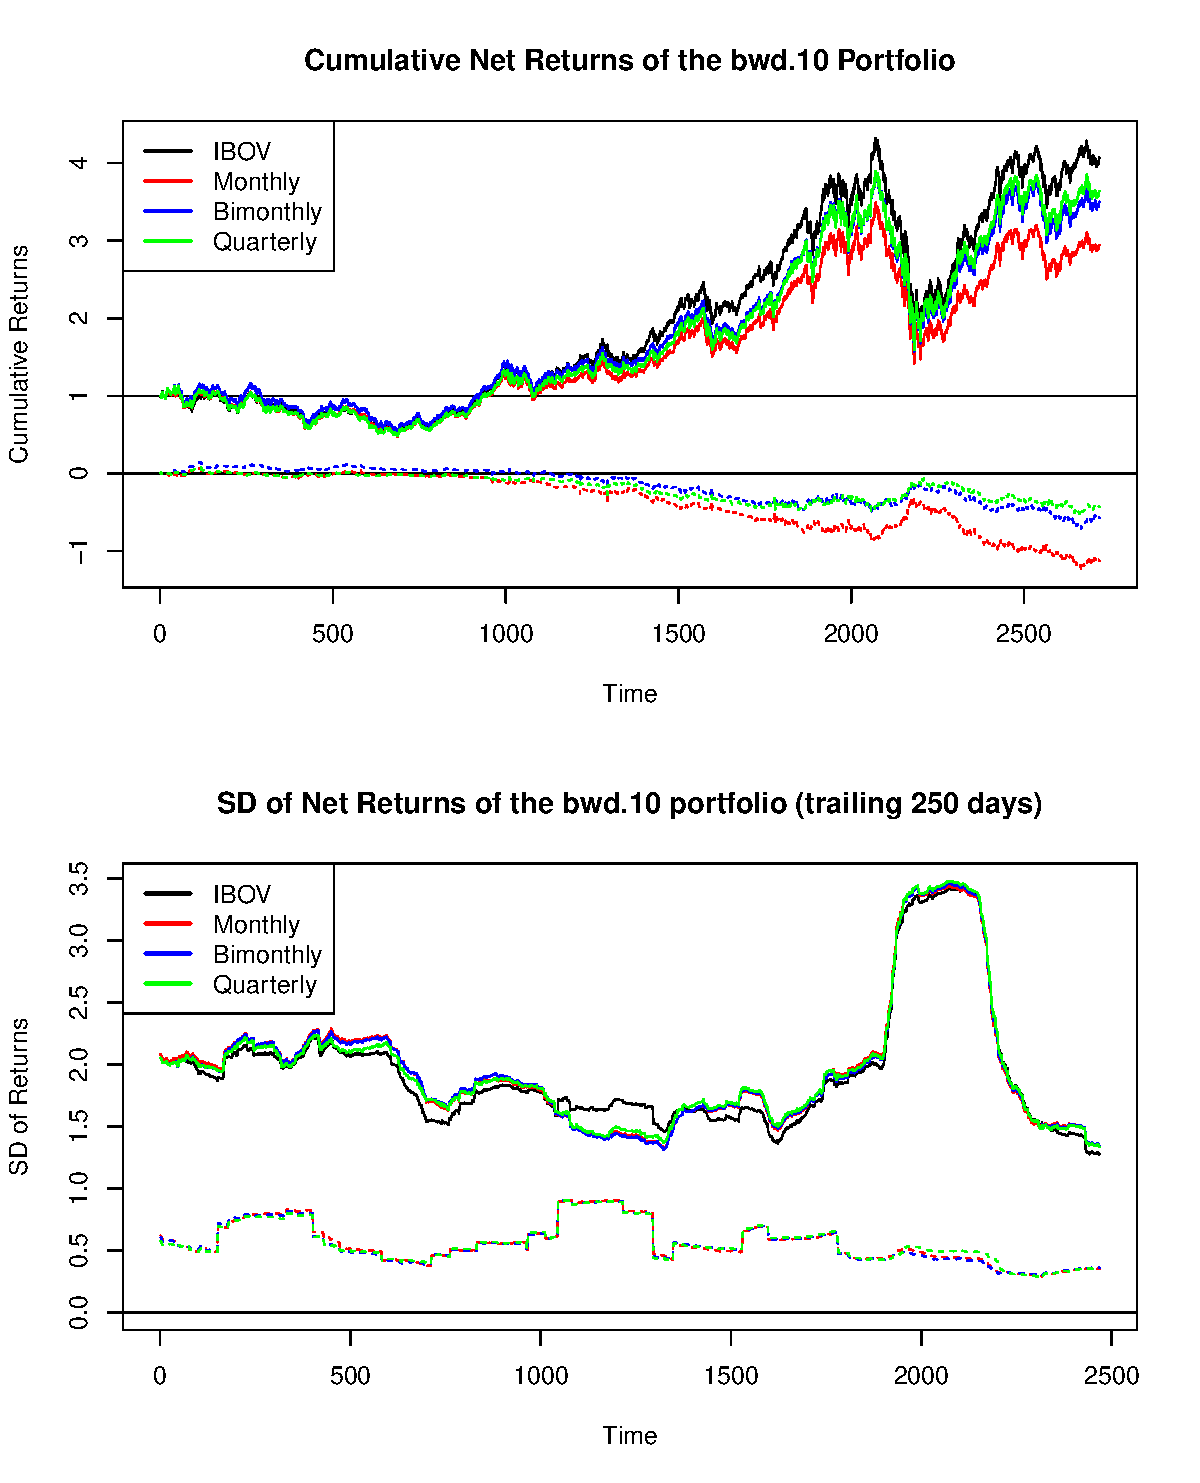
\includegraphics[width=.95\linewidth]{./figs/IBOV-retac-bwd-10.pdf}
\begin{quote}
\textbf{Source:} The author.
\end{quote}
\end{figure}

\begin{figure}[htpb]
\centering
\footnotesize
\caption{\texttt{bwd.15} Portfolio (Brazilian Data)}
\label{fig:ibov:bwd.15}
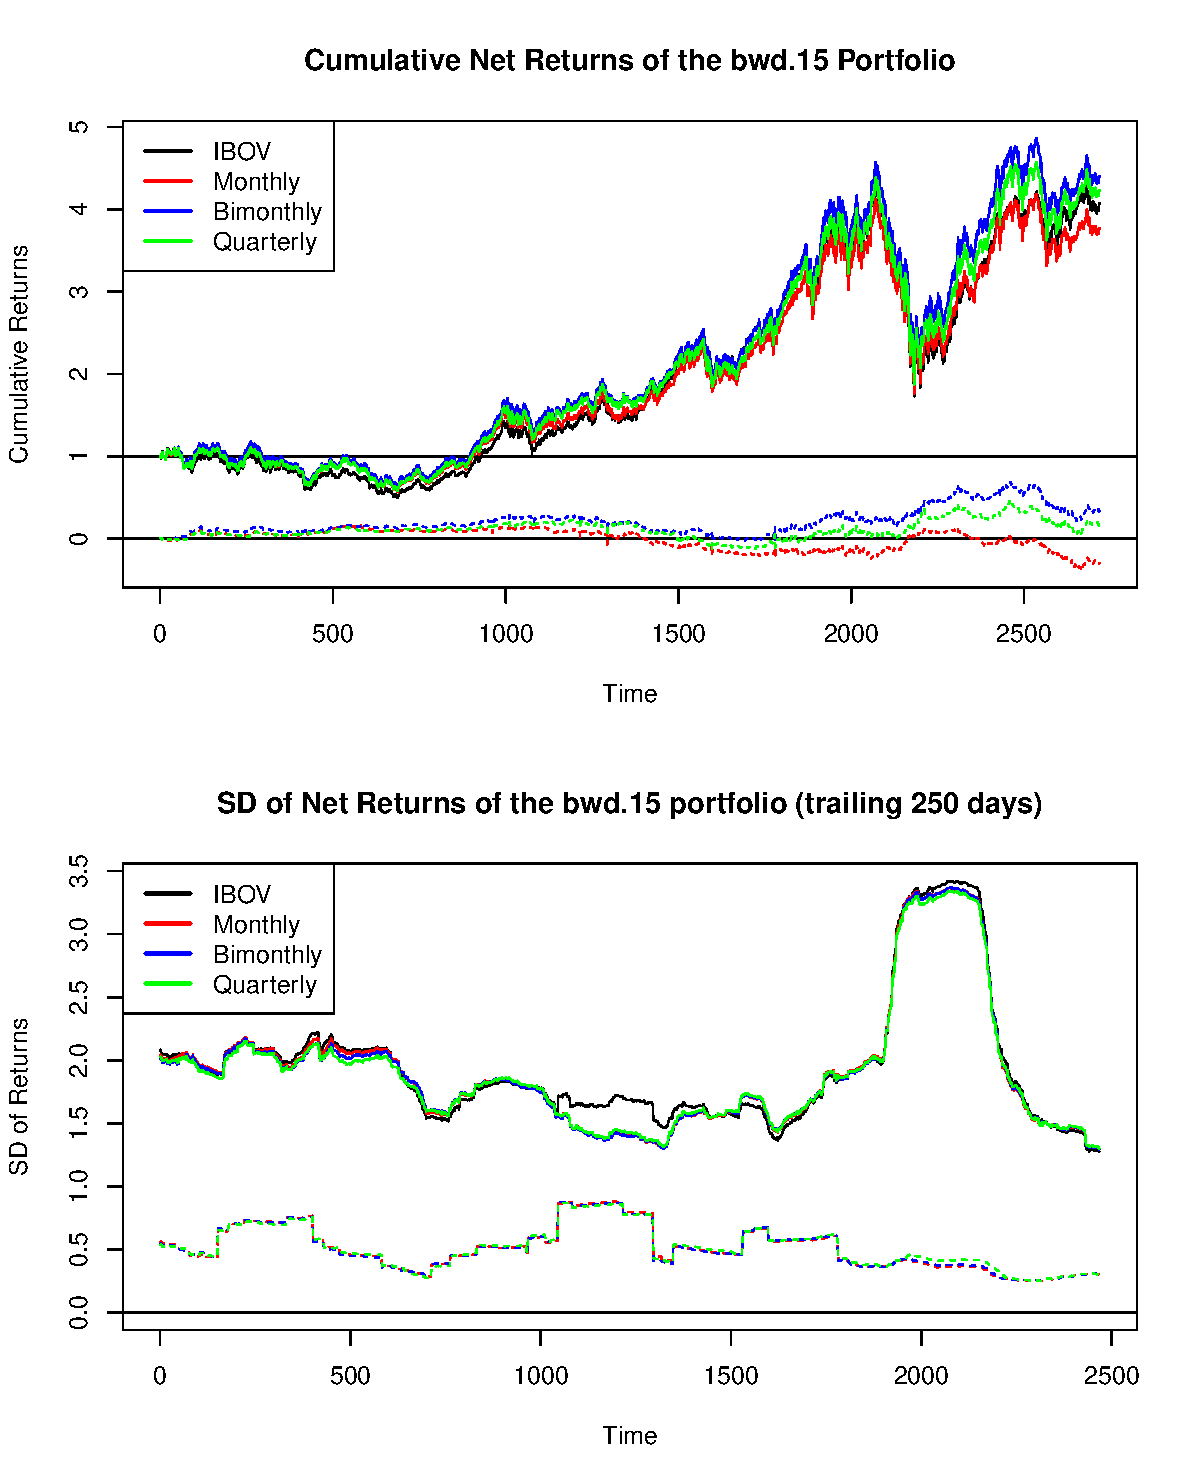
\includegraphics[width=.95\linewidth]{./figs/IBOV-retac-bwd-15.pdf}
\begin{quote}
\textbf{Source:} The author.
\end{quote}
\end{figure}

\begin{figure}[htpb]
\centering
\footnotesize
\caption{\texttt{bwd.20} Portfolio (Brazilian Data)}
\label{fig:ibov:bwd.20}
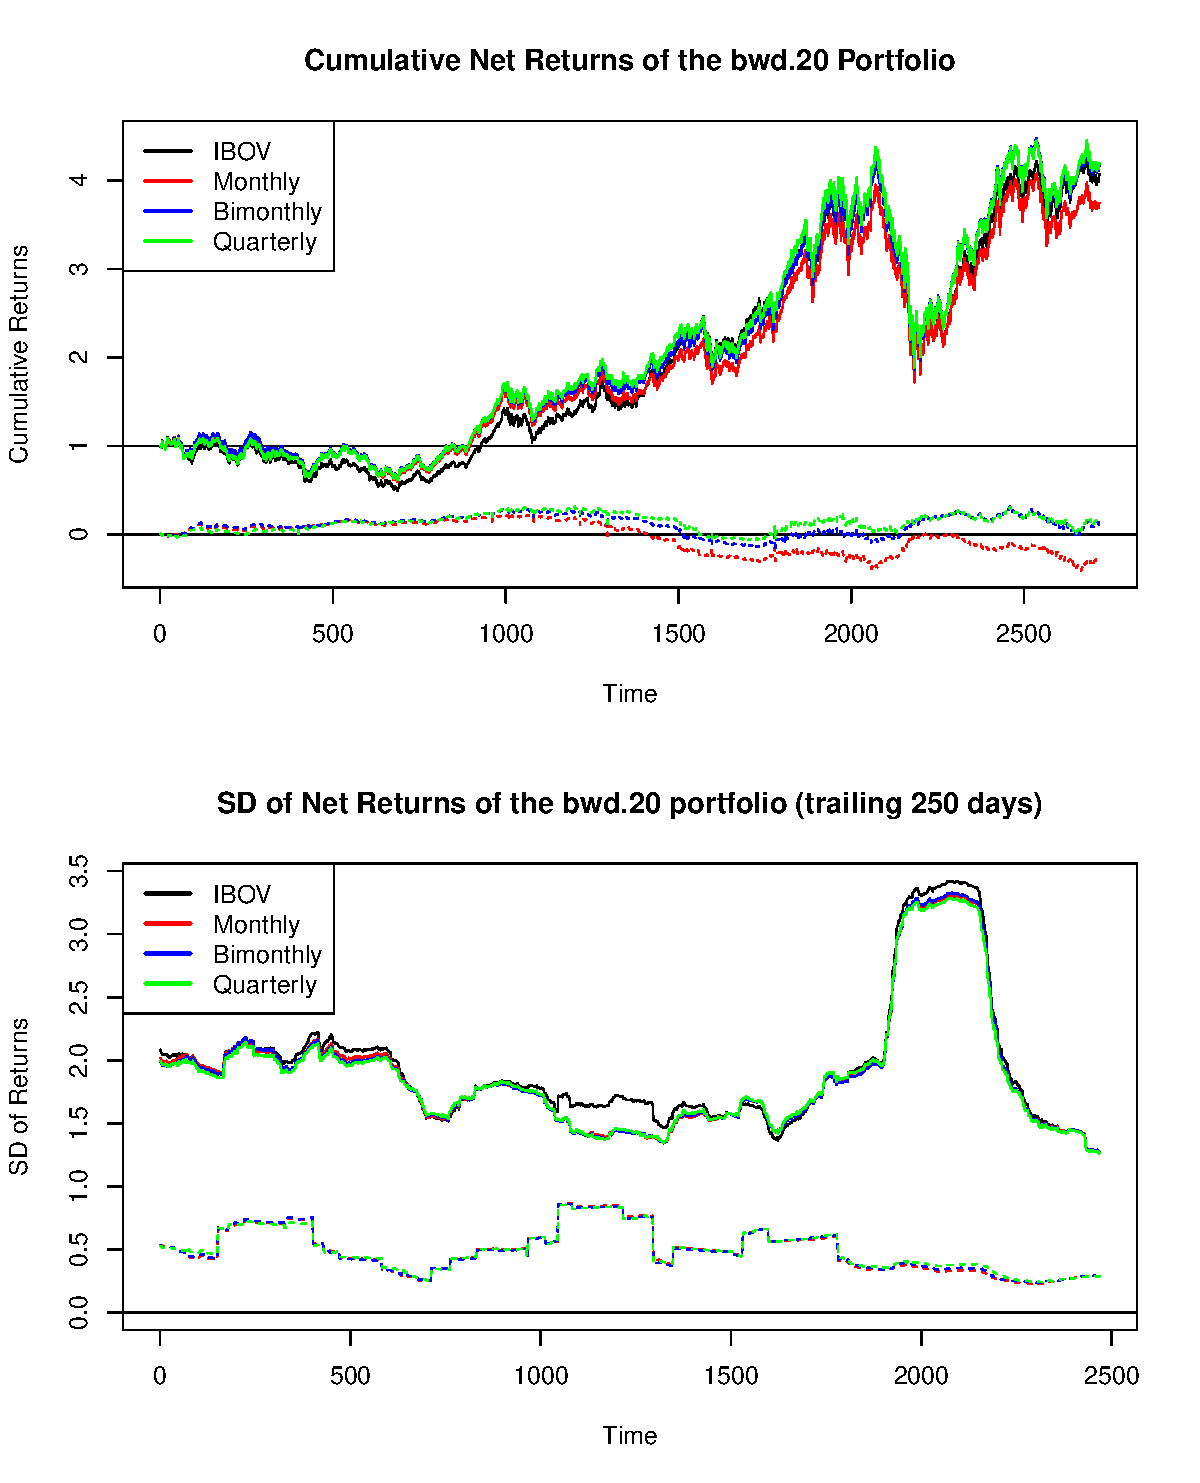
\includegraphics[width=.95\linewidth]{./figs/IBOV-retac-bwd-20.pdf}
\begin{quote}
\textbf{Source:} The author.
\end{quote}
\end{figure}

%%%%%%%%%%%%%%%%%%%%%%%%%%%%%%%%%%%%%%%%%%%%%%%%%%%%%%%%%%%%%%%%%
\begin{figure}[htpb]
\centering
\footnotesize
\caption{\texttt{fwd.10} Portfolio (Brazilian Data)}
\label{fig:ibov:fwd.10}
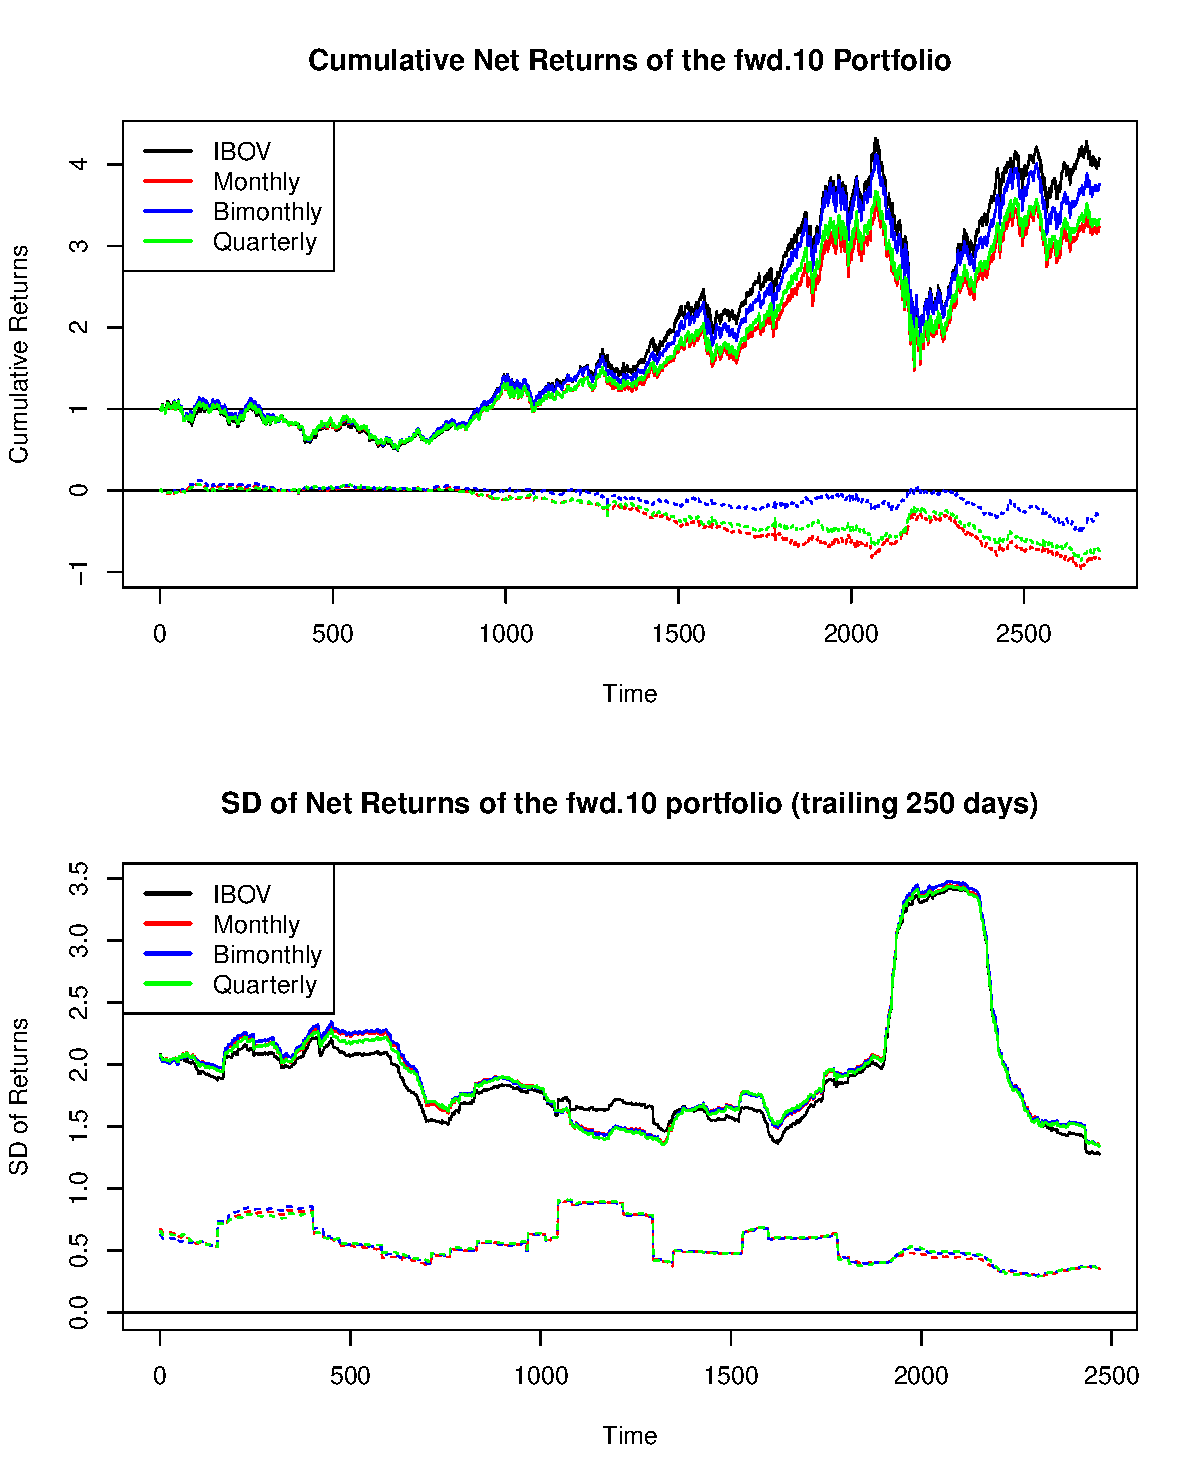
\includegraphics[width=.95\linewidth]{./figs/IBOV-retac-fwd-10.pdf}
\begin{quote}
\textbf{Source:} The author.
\end{quote}
\end{figure}

\begin{figure}[htpb]
\centering
\footnotesize
\caption{\texttt{fwd.15} Portfolio (Brazilian Data)}
\label{fig:ibov:fwd.15}
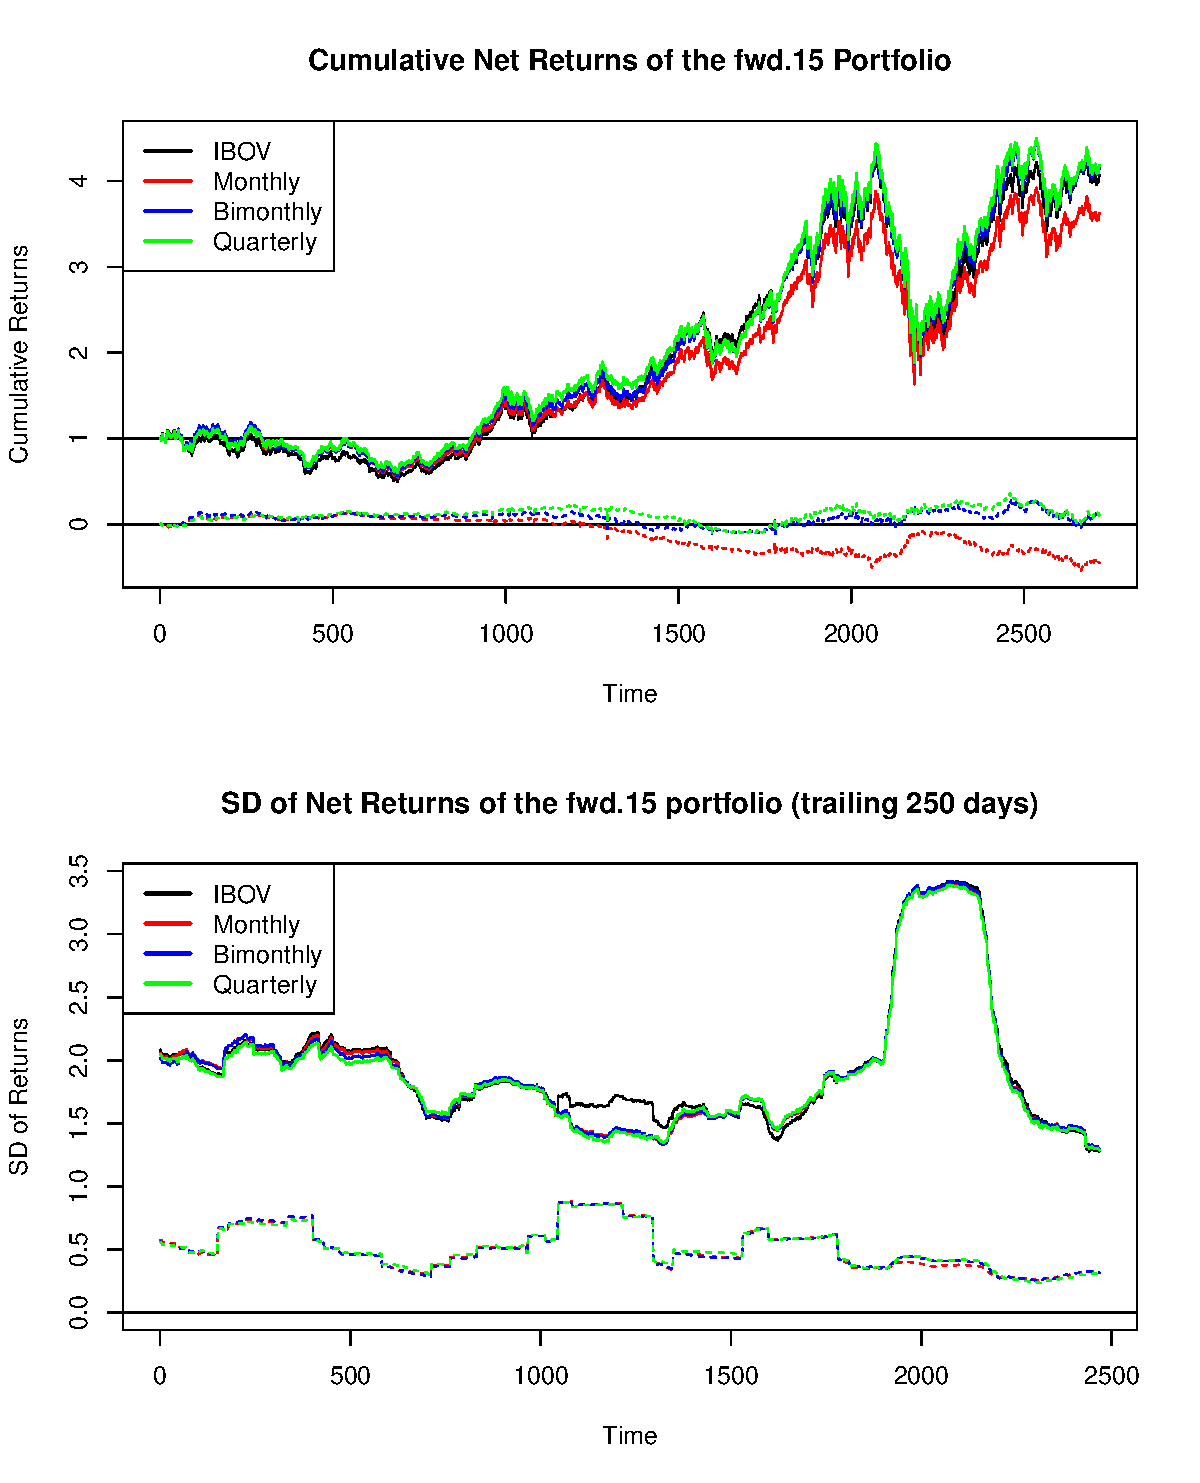
\includegraphics[width=.95\linewidth]{./figs/IBOV-retac-fwd-15.pdf}
\begin{quote}
\textbf{Source:} The author.
\end{quote}
\end{figure}

\begin{figure}[htpb]
\centering
\footnotesize
\caption{\texttt{fwd.20} Portfolio (Brazilian Data)}
\label{fig:ibov:fwd.20}
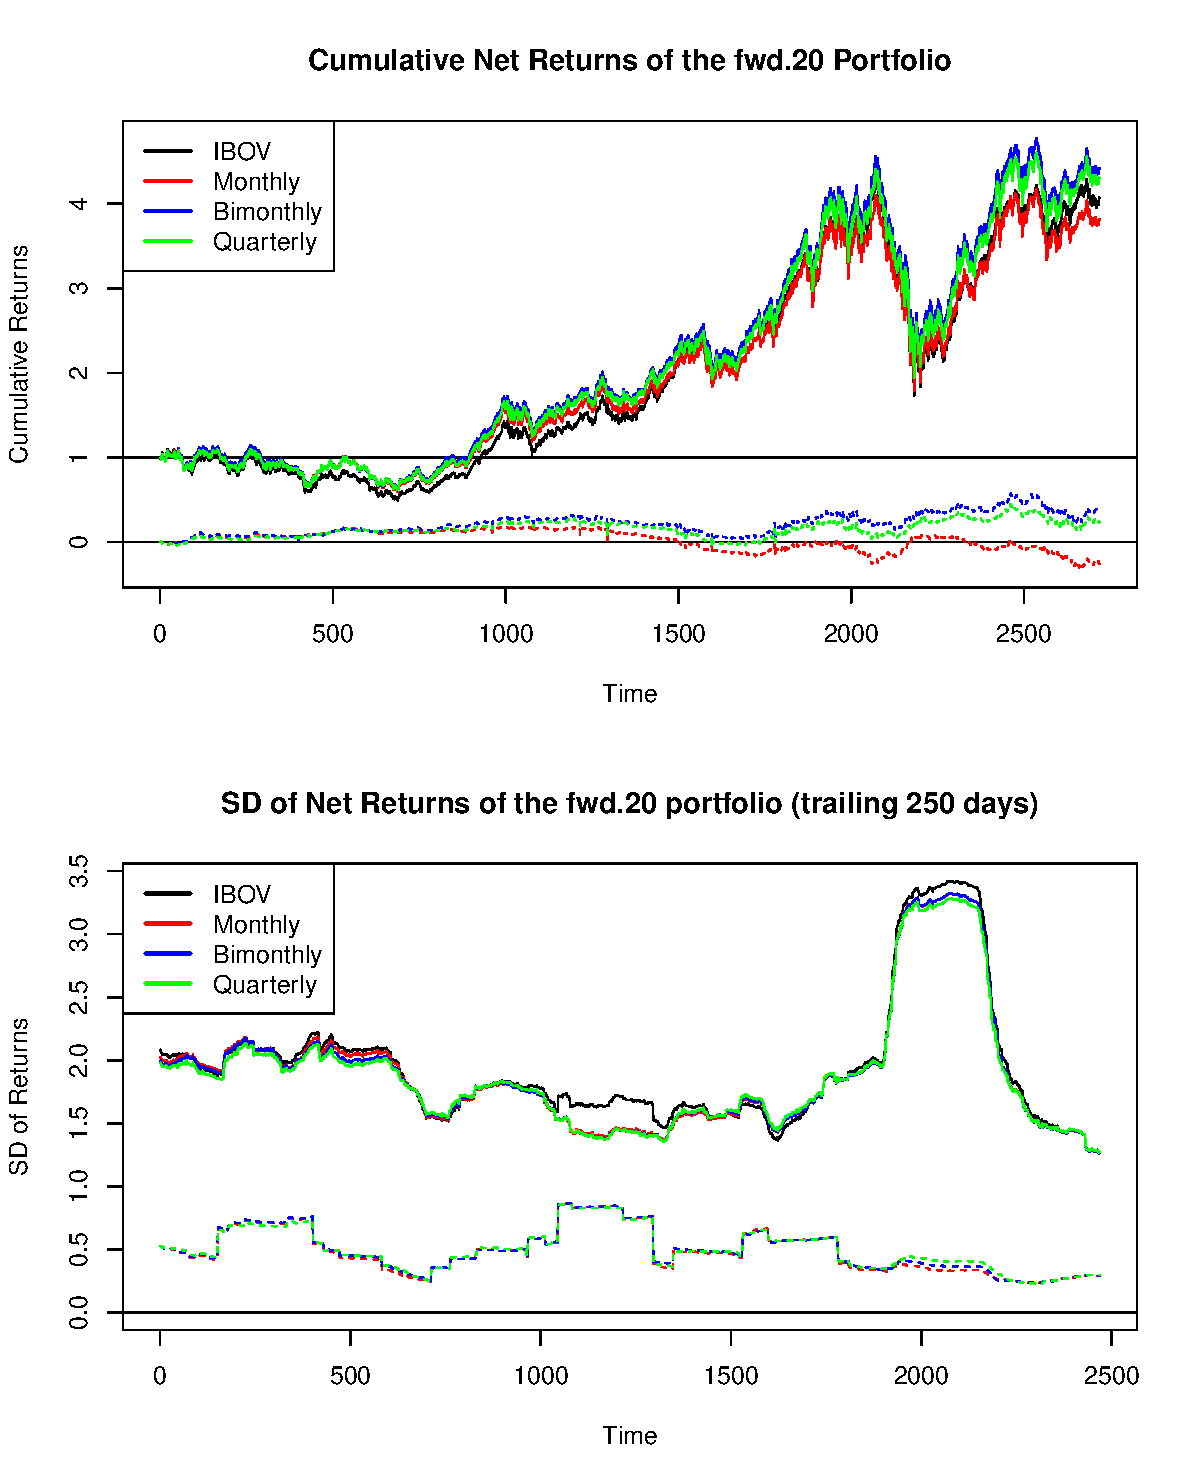
\includegraphics[width=.95\linewidth]{./figs/IBOV-retac-fwd-20.pdf}
\begin{quote}
\textbf{Source:} The author.
\end{quote}
\end{figure}

%%%%%%%%%%%%%%%%%%%%%%%%%%%%%%%%%%%%%%%%%%%%%%%%%%%%%%%%%%%%%%%%%
% lasso ibov
\begin{figure}[htpb]
\centering
\footnotesize
\caption{\texttt{las.10} Portfolio (Brazilian Data)}
\label{fig:ibov:las.10}
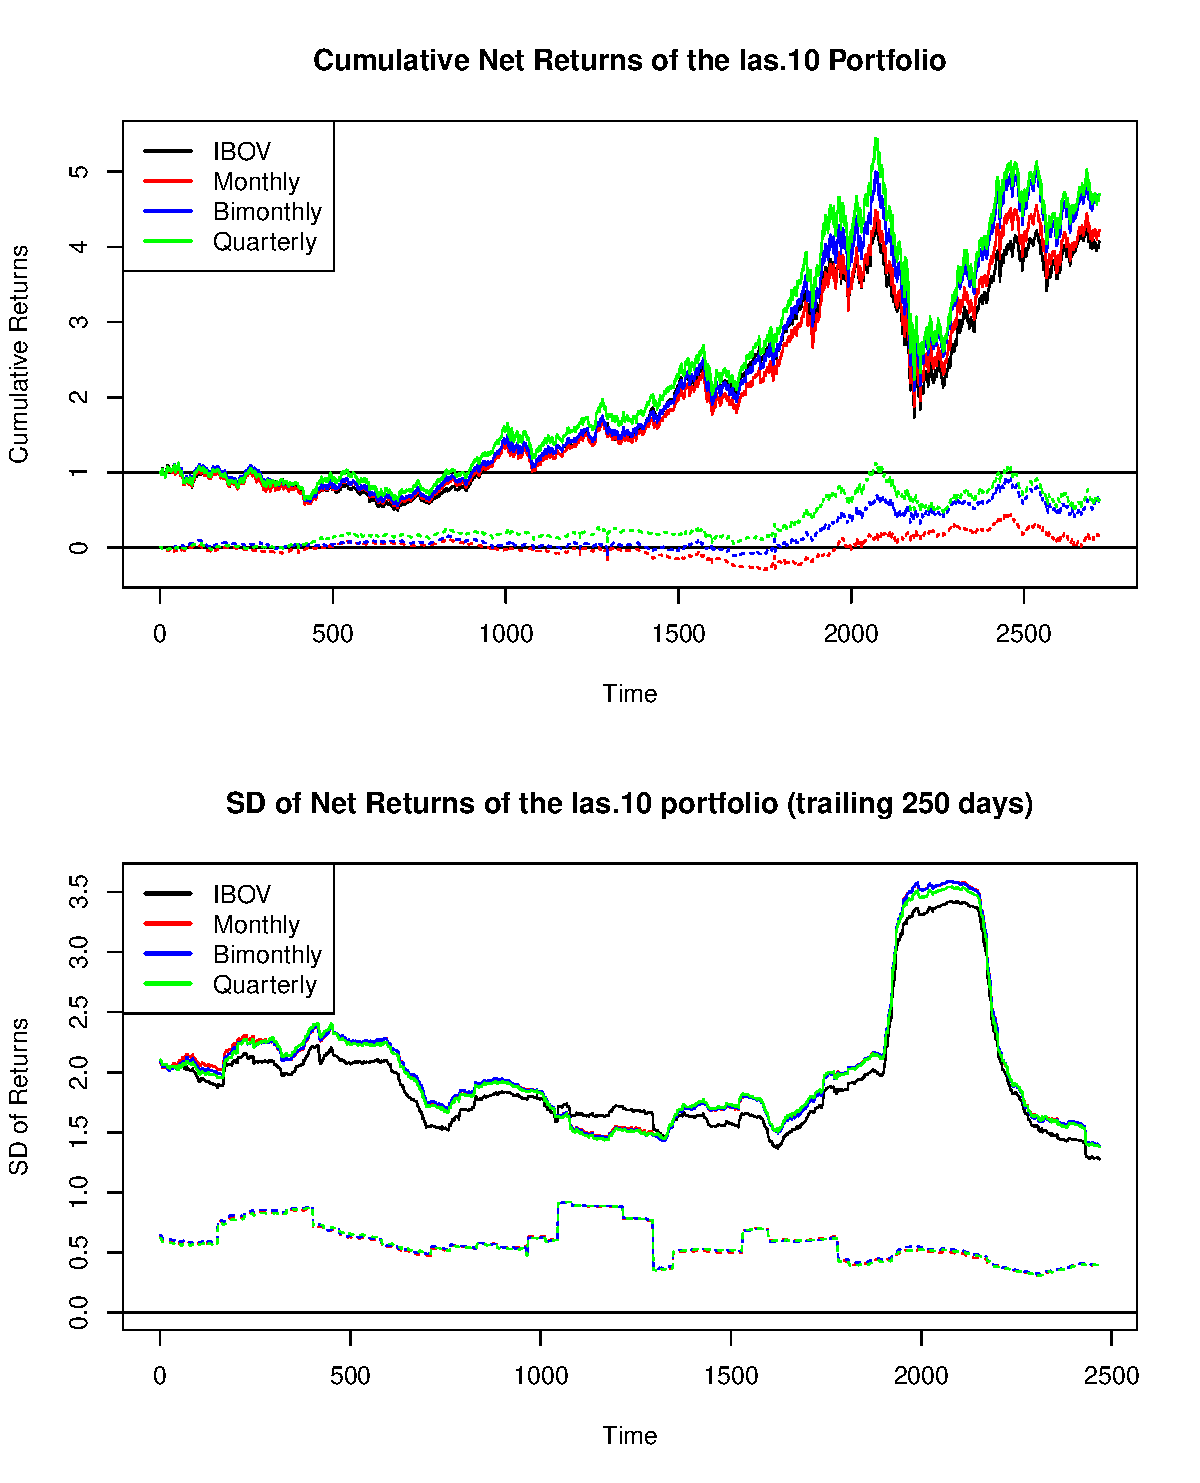
\includegraphics[width=.95\linewidth]{./figs/IBOV-retac-las-10.pdf}
\begin{quote}
\textbf{Source:} The author.
\end{quote}
\end{figure}

\begin{figure}[htpb]
\centering
\footnotesize
\caption{\texttt{las.15} Portfolio (Brazilian Data)}
\label{fig:ibov:las.15}
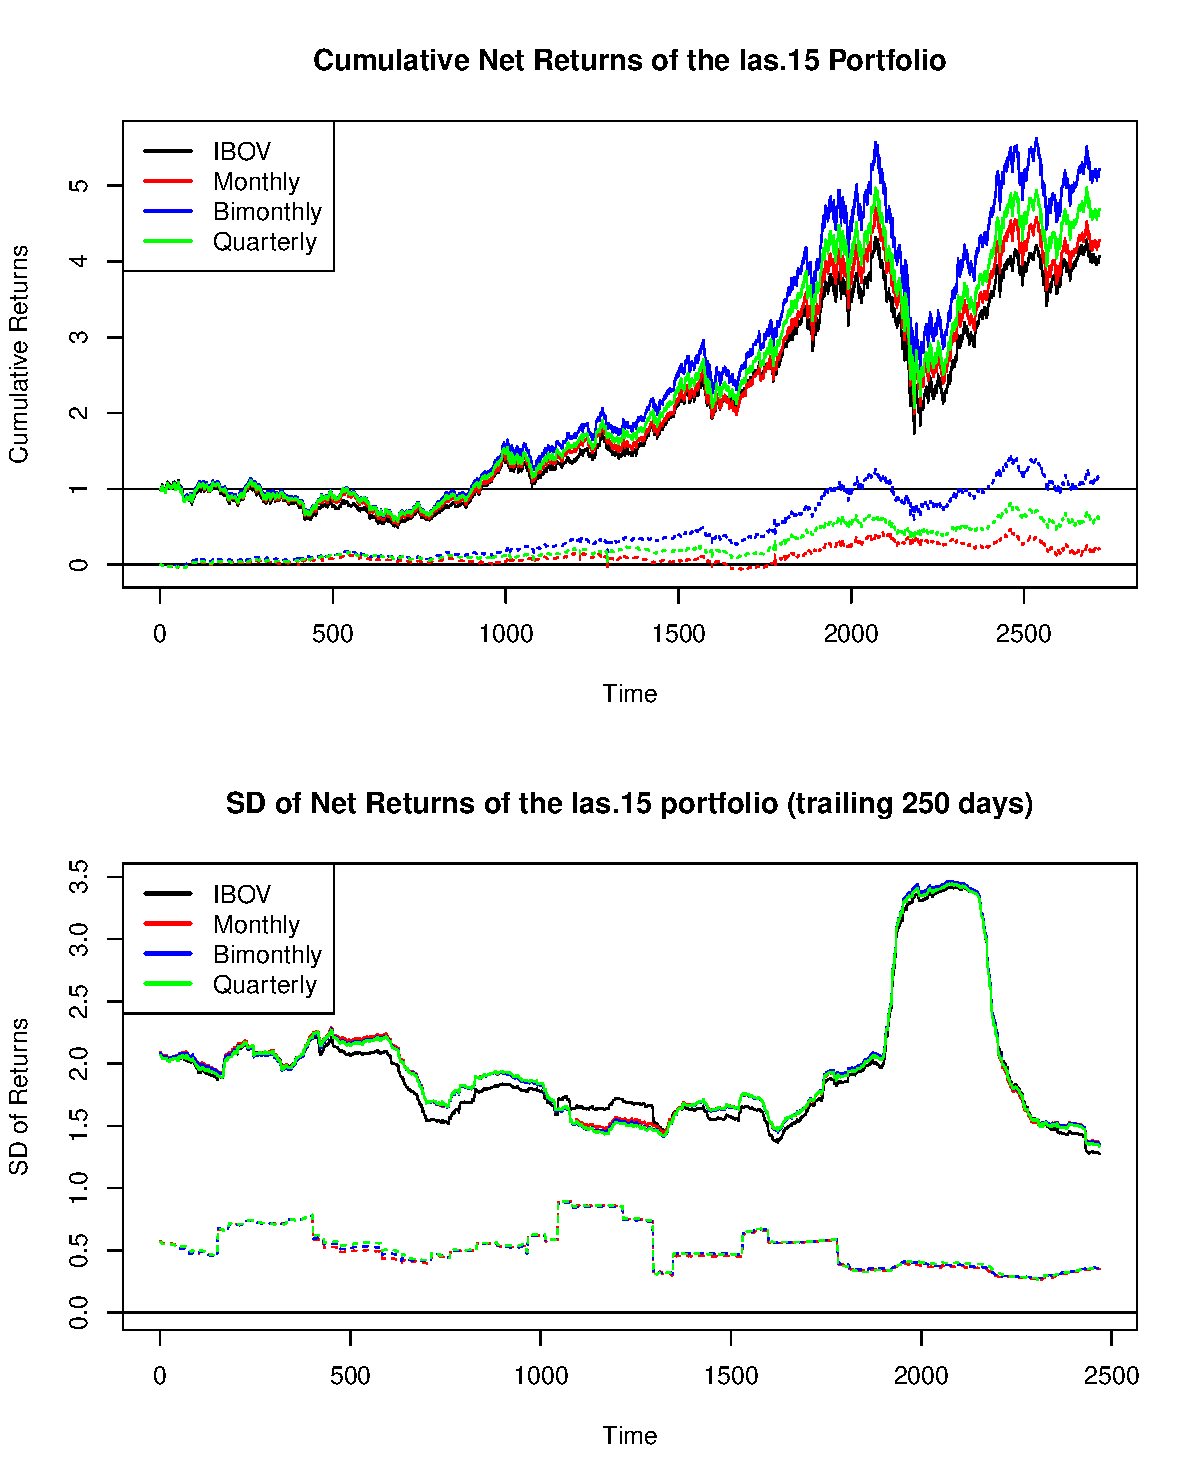
\includegraphics[width=.95\linewidth]{./figs/IBOV-retac-las-15.pdf}
\begin{quote}
\textbf{Source:} The author.
\end{quote}
\end{figure}

\begin{figure}[htpb]
\centering
\footnotesize
\caption{\texttt{las.20} Portfolio (Brazilian Data)}
\label{fig:ibov:las.20}
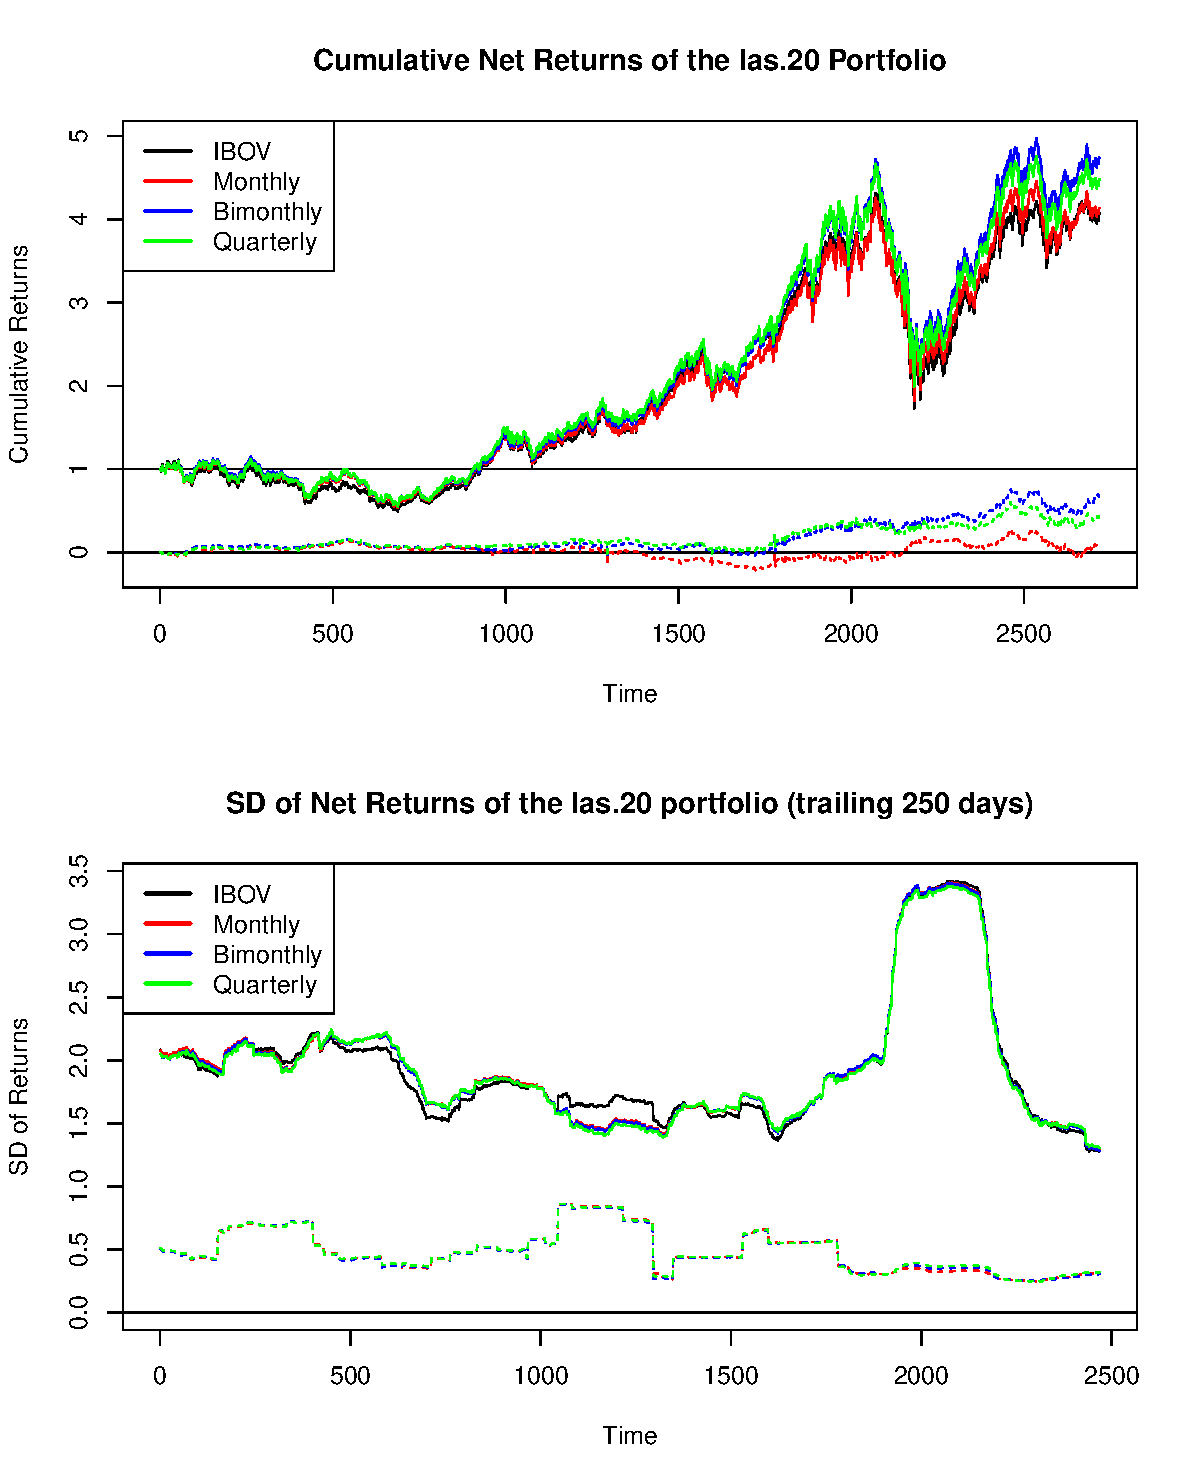
\includegraphics[width=.95\linewidth]{./figs/IBOV-retac-las-20.pdf}
\begin{quote}
\textbf{Source:} The author.
\end{quote}
\end{figure}


%%%%%%%%%%%%%%%%%%%%%%%%%%%%%%%%%%%%%%%%%%%%%%%%%%%%%%%%%%%%%%%%%
% SP500 TABS
\clearpage
\input{./tabs/spy5-rps.tex}
% pvals % RPN
\input{./tabs/pval-sr-rpn-spy5.tex}
\input{./tabs/pval-var-rpn-spy5.tex}
\input{./tabs/pval-mu-rpn-spy5.tex}

%%%%%%%%%%%%%%%%%%%%%%%%%%%%%%%%%%%%%%%%%%%%%%%%%%%%%%%%%%%%%%%%%%%%%%%%%%%%%%%%%%%%
% SPY FIGS
\clearpage

%%%%%%%%%%%%%%%%%%%%%%%%%%%%%%%%%%%%%%%%%%%%%%%%%%%%%%%%%%%%%%%%%%%%%%%%%%%%%%%%%%%%
% SPY BWD 

\begin{figure}[htpb]
\centering
\footnotesize
\caption{\texttt{bwd.20} Portfolio (American Data)}
\label{fig:spy:bwd.20}
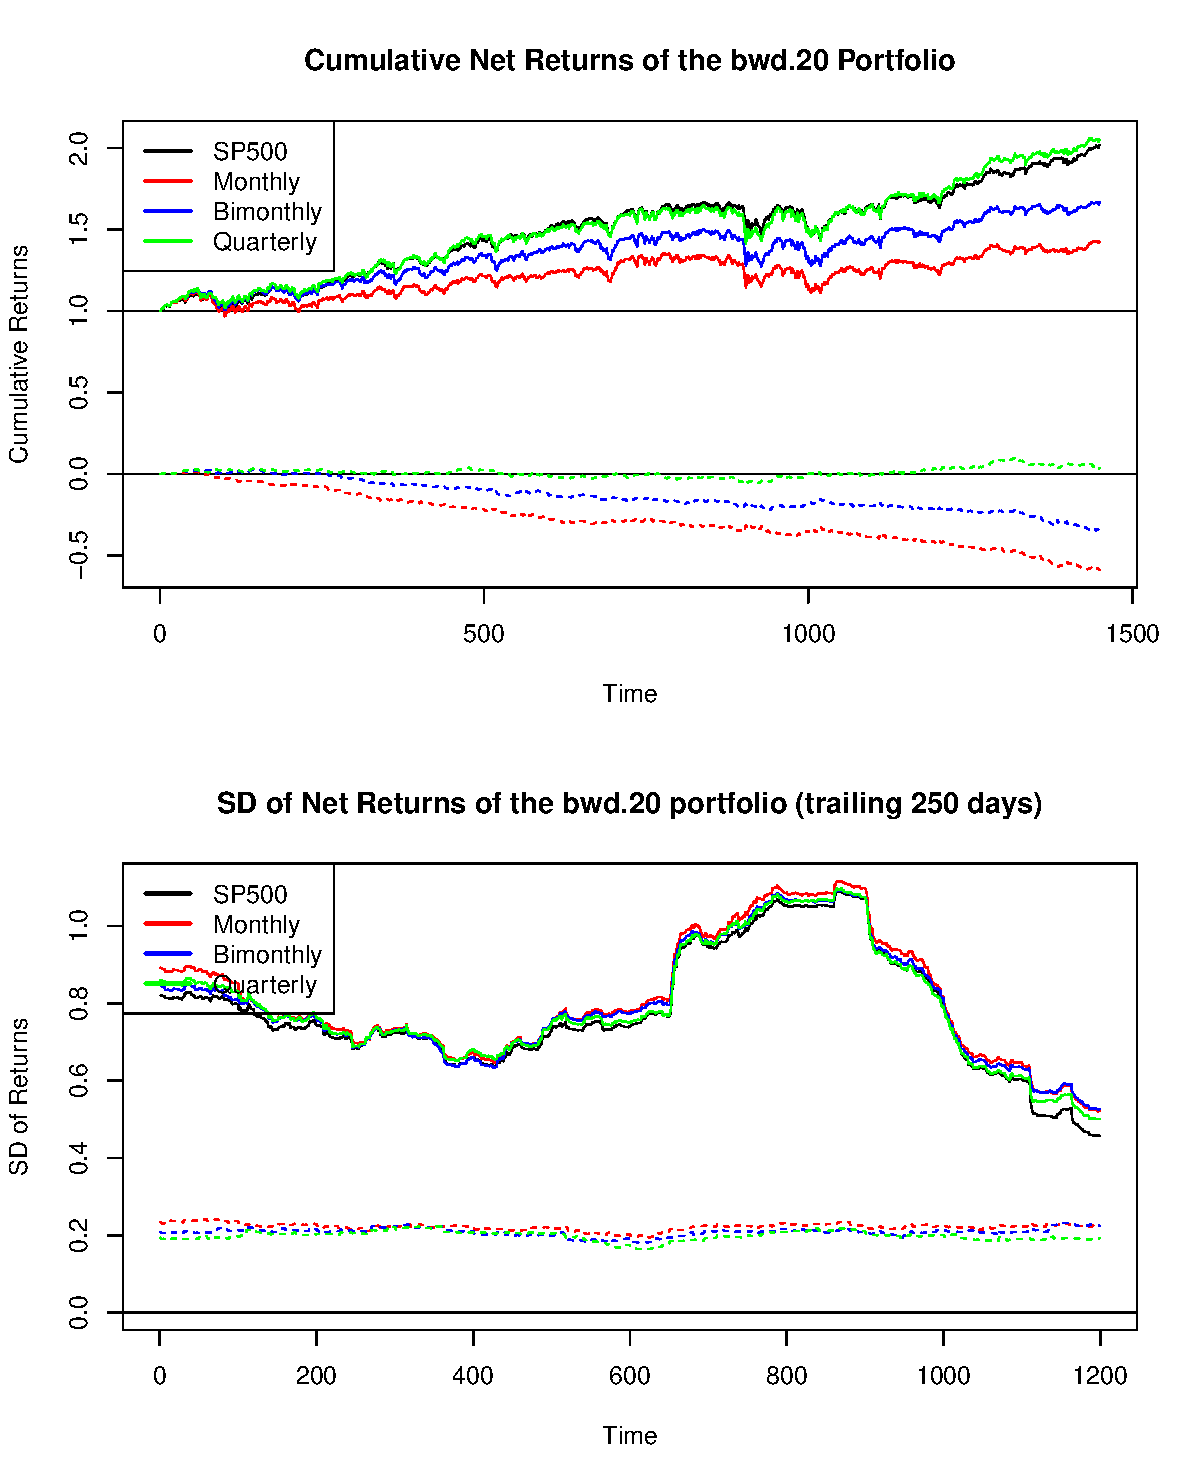
\includegraphics[width=.95\linewidth]{./figs/SP500-retac-bwd-20.pdf}
\begin{quote}
\textbf{Source:} The author.
\end{quote}
\end{figure}

\begin{figure}[htpb]
\centering
\footnotesize
\caption{\texttt{bwd.30} Portfolio (American Data)}
\label{fig:spy:bwd.30}
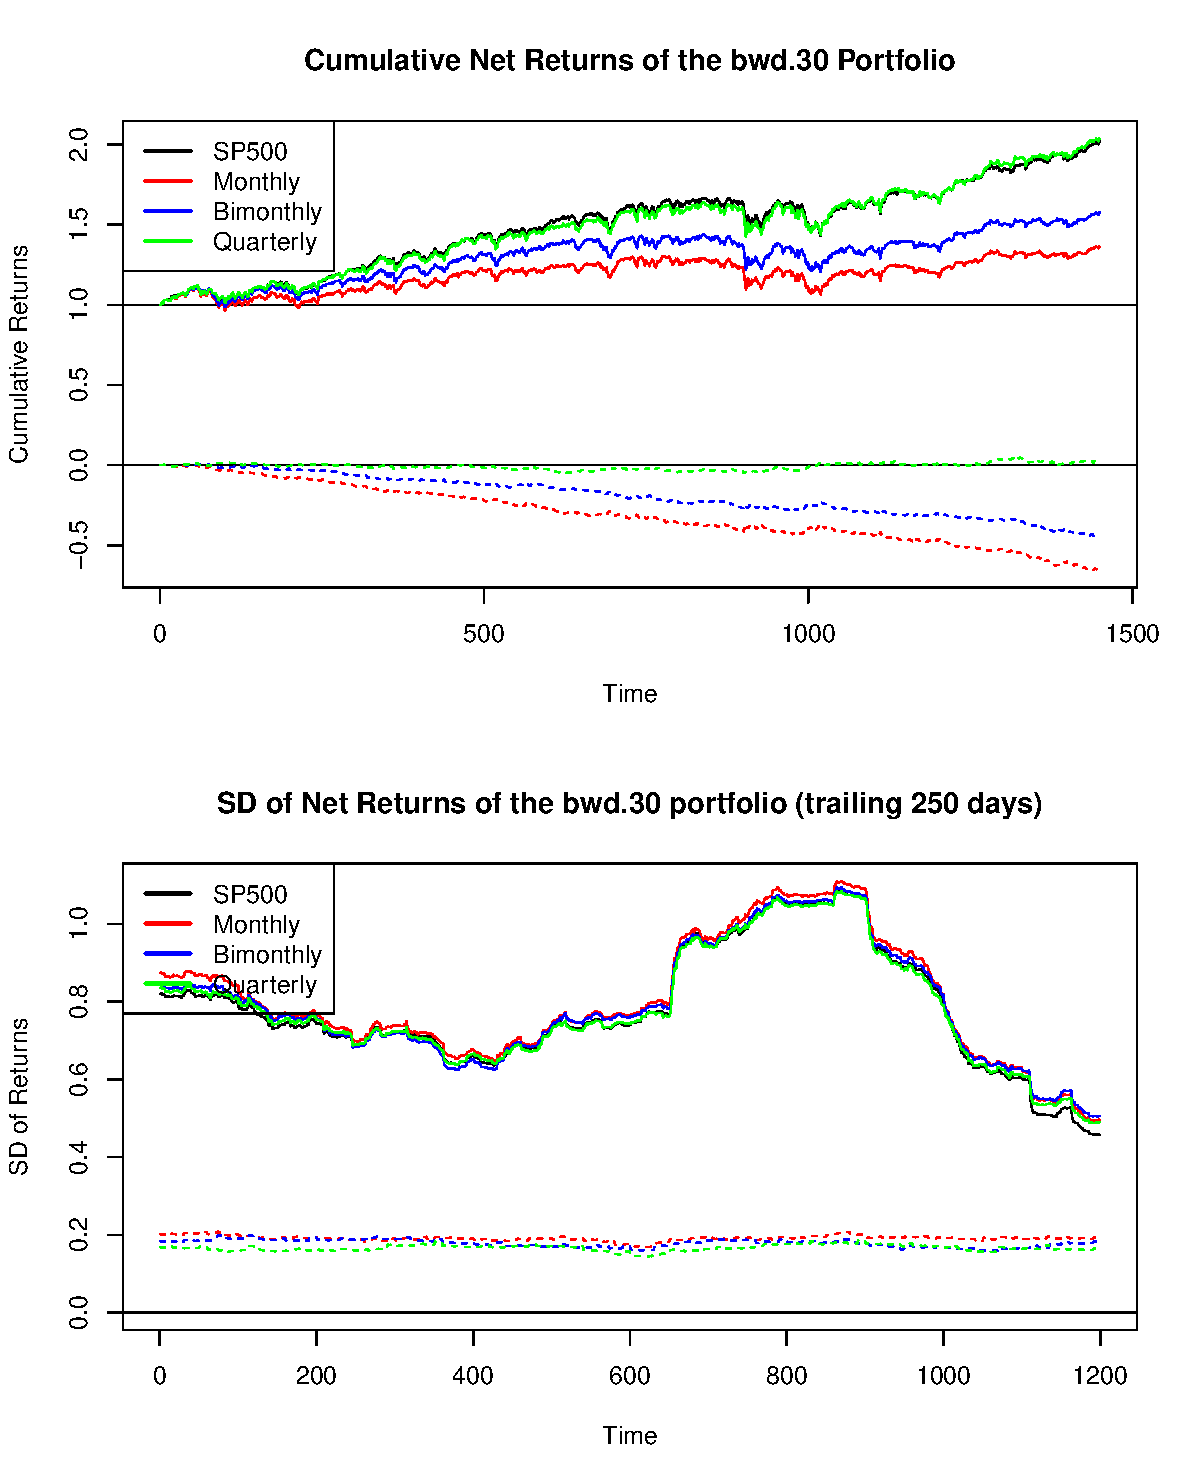
\includegraphics[width=.95\linewidth]{./figs/SP500-retac-bwd-30.pdf}
\begin{quote}
\textbf{Source:} The author.
\end{quote}
\end{figure}

\begin{figure}[htpb]
\centering
\footnotesize
\caption{\texttt{bwd.40} Portfolio (American Data)}
\label{fig:spy:bwd.40}
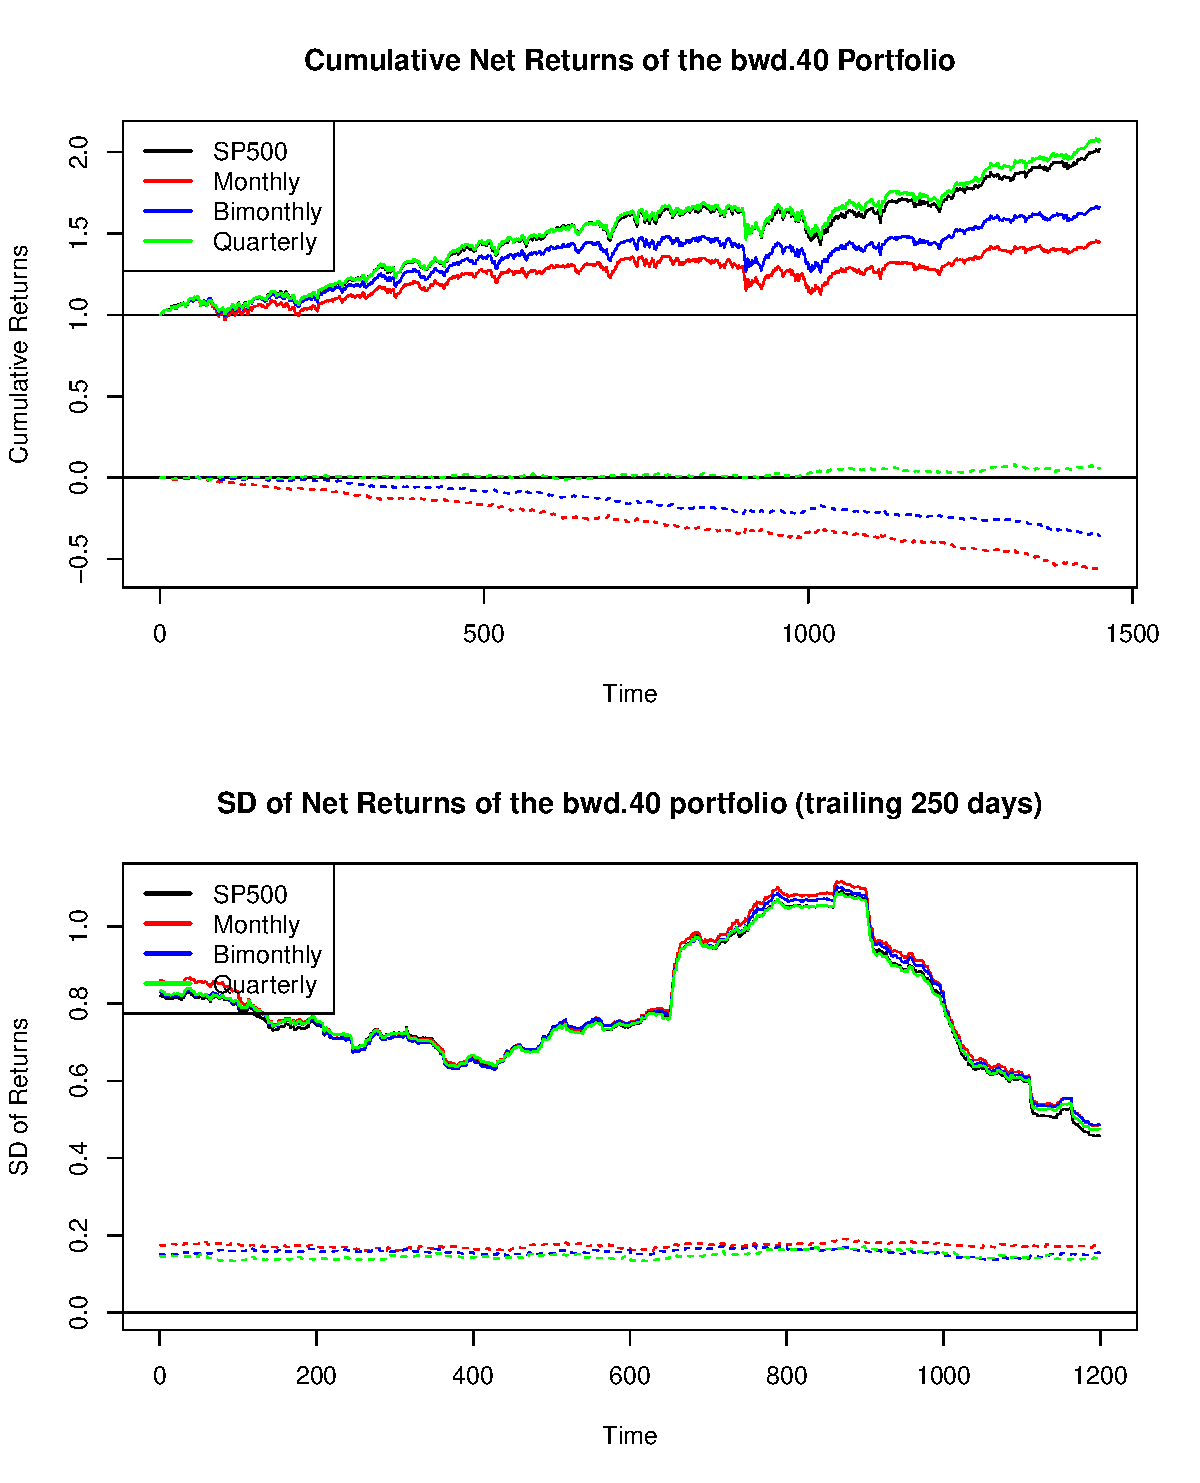
\includegraphics[width=.95\linewidth]{./figs/SP500-retac-bwd-40.pdf}
\begin{quote}
\textbf{Source:} The author.
\end{quote}
\end{figure}
%%%%%%%%%%%%%%%%%%%%%%%%%%%%%%%%%%%%%%%%%%%%%%%%%%%%%%%%%%%%%%%%%%%%%%%%%%%%%%%%%%%%
% SPY FWD 

\begin{figure}[htpb]
\centering
\footnotesize
\caption{\texttt{fwd.20} Portfolio (American Data)}
\label{fig:spy:fwd.20}
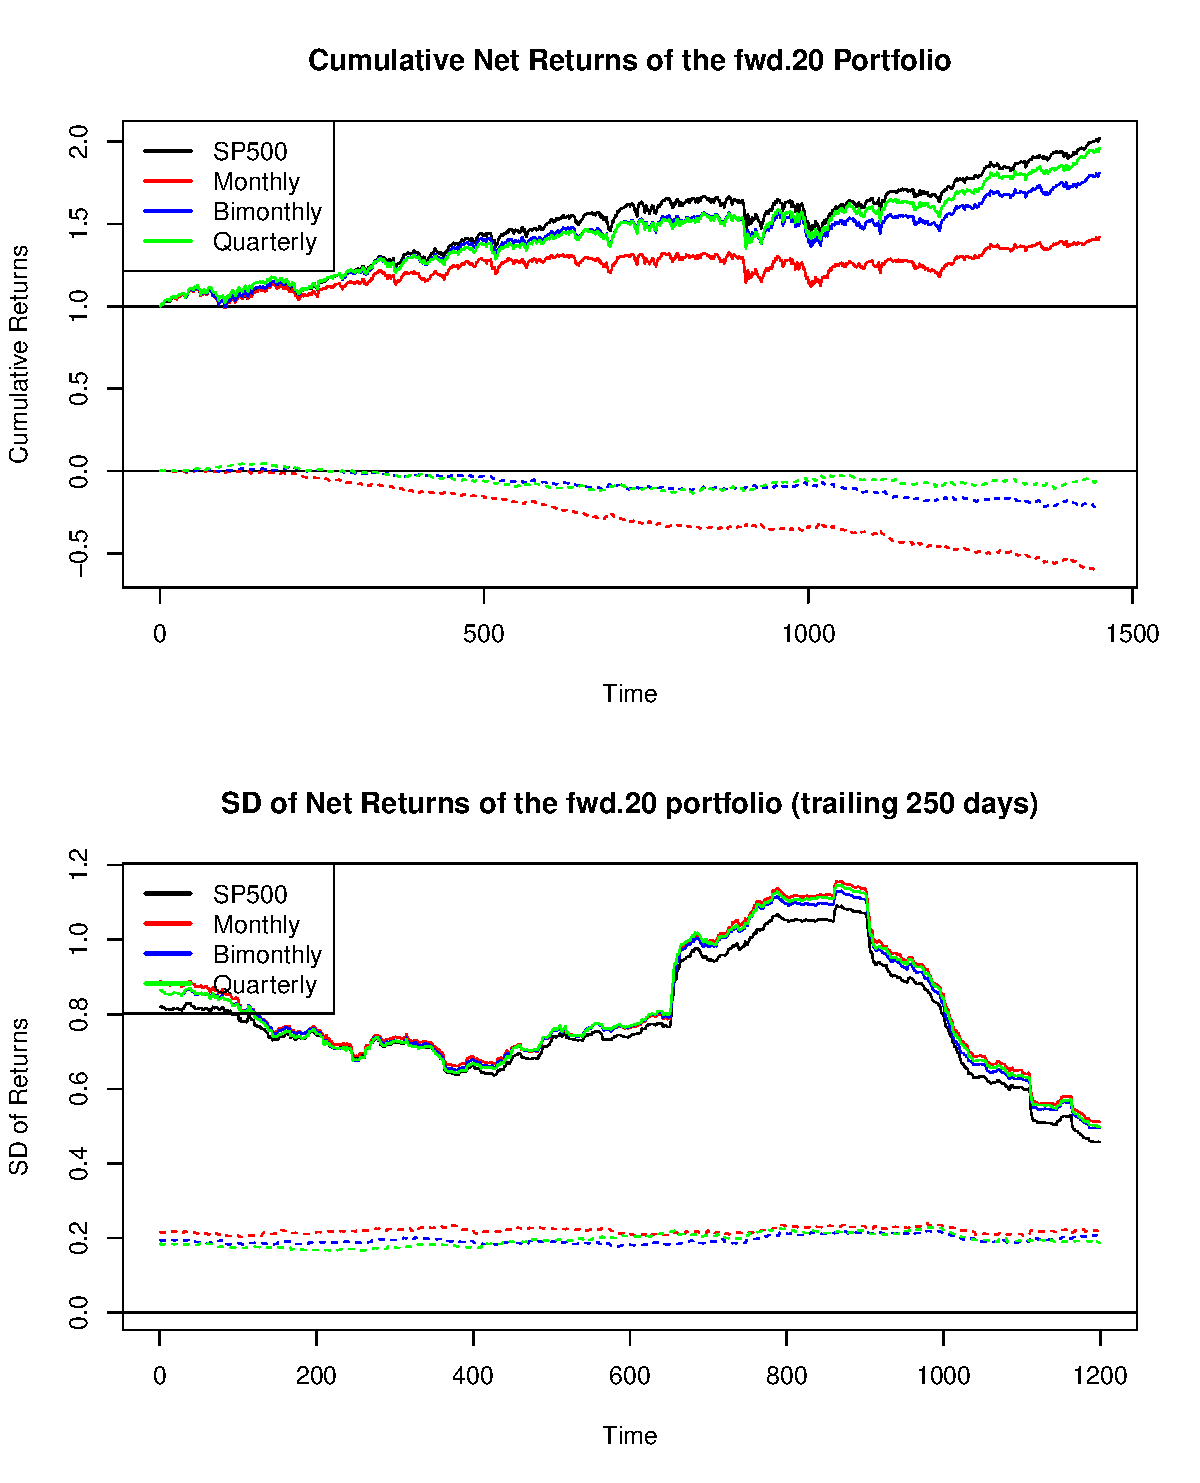
\includegraphics[width=.95\linewidth]{./figs/SP500-retac-fwd-20.pdf}
\begin{quote}
\textbf{Source:} The author.
\end{quote}
\end{figure}

\begin{figure}[htpb]
\centering
\footnotesize
\caption{\texttt{fwd.30} Portfolio (American Data)}
\label{fig:spy:fwd.30}
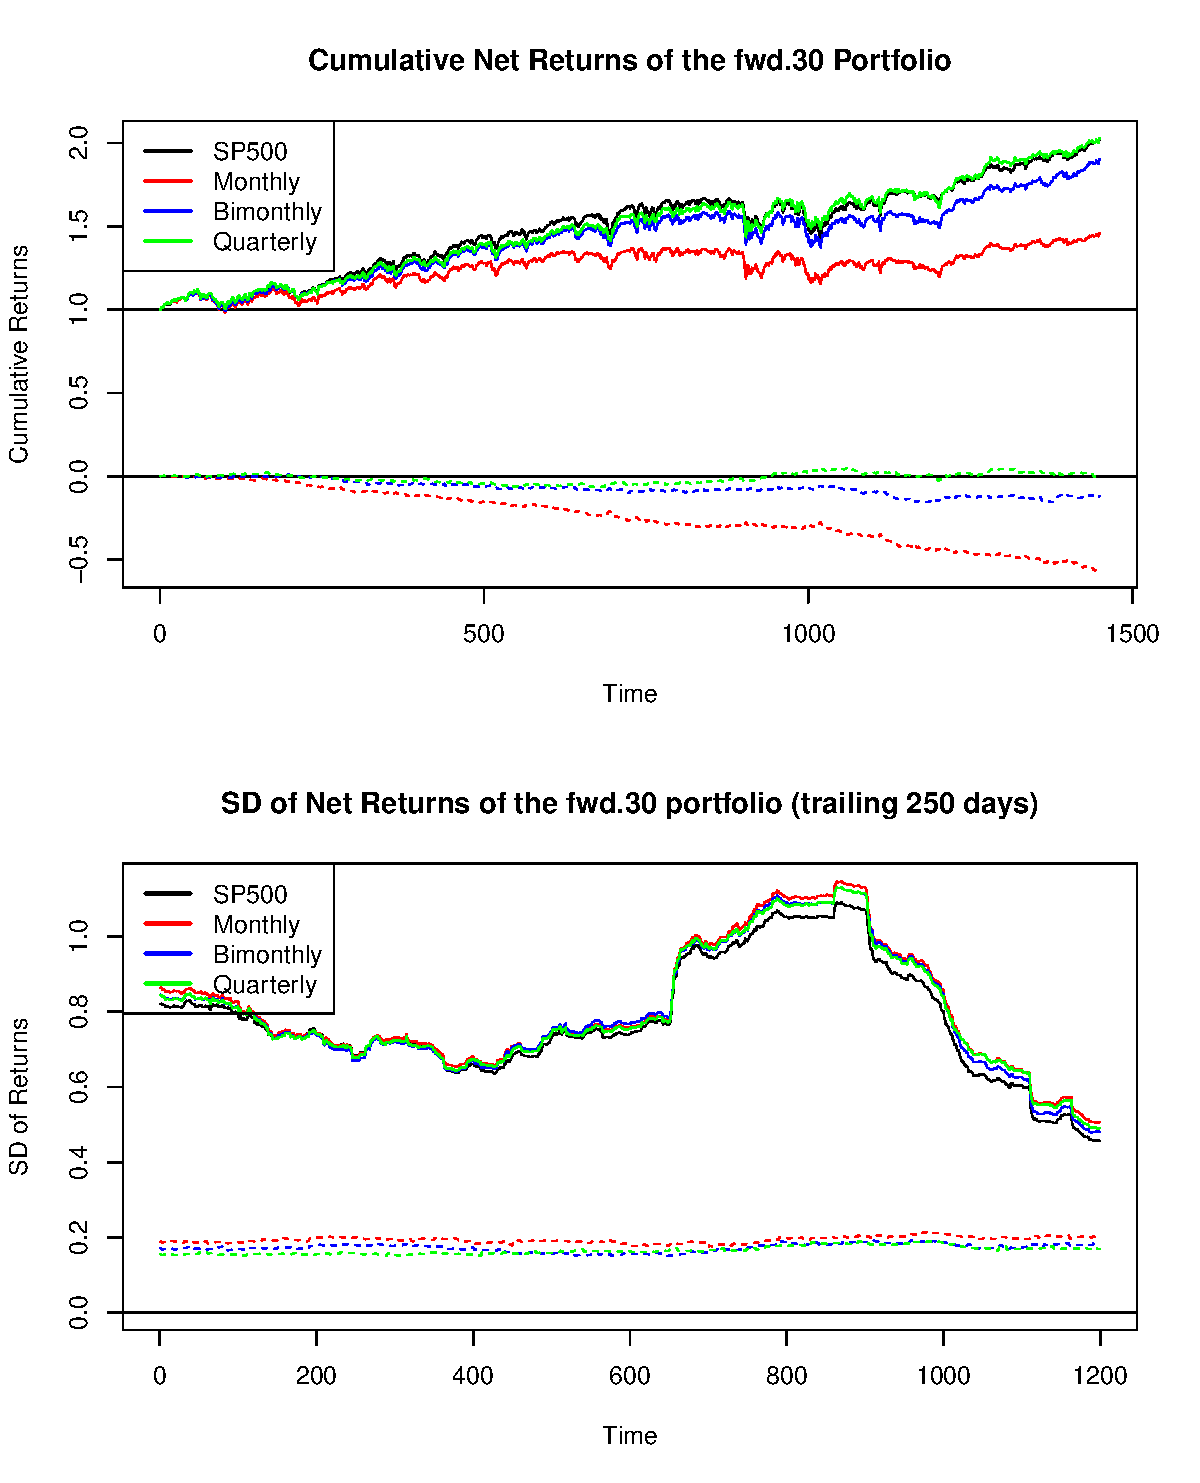
\includegraphics[width=.95\linewidth]{./figs/SP500-retac-fwd-30.pdf}
\begin{quote}
\textbf{Source:} The author.
\end{quote}
\end{figure}

\begin{figure}[htpb]
\centering
\footnotesize
\caption{\texttt{fwd.40} Portfolio (American Data)}
\label{fig:spy:fwd.40}
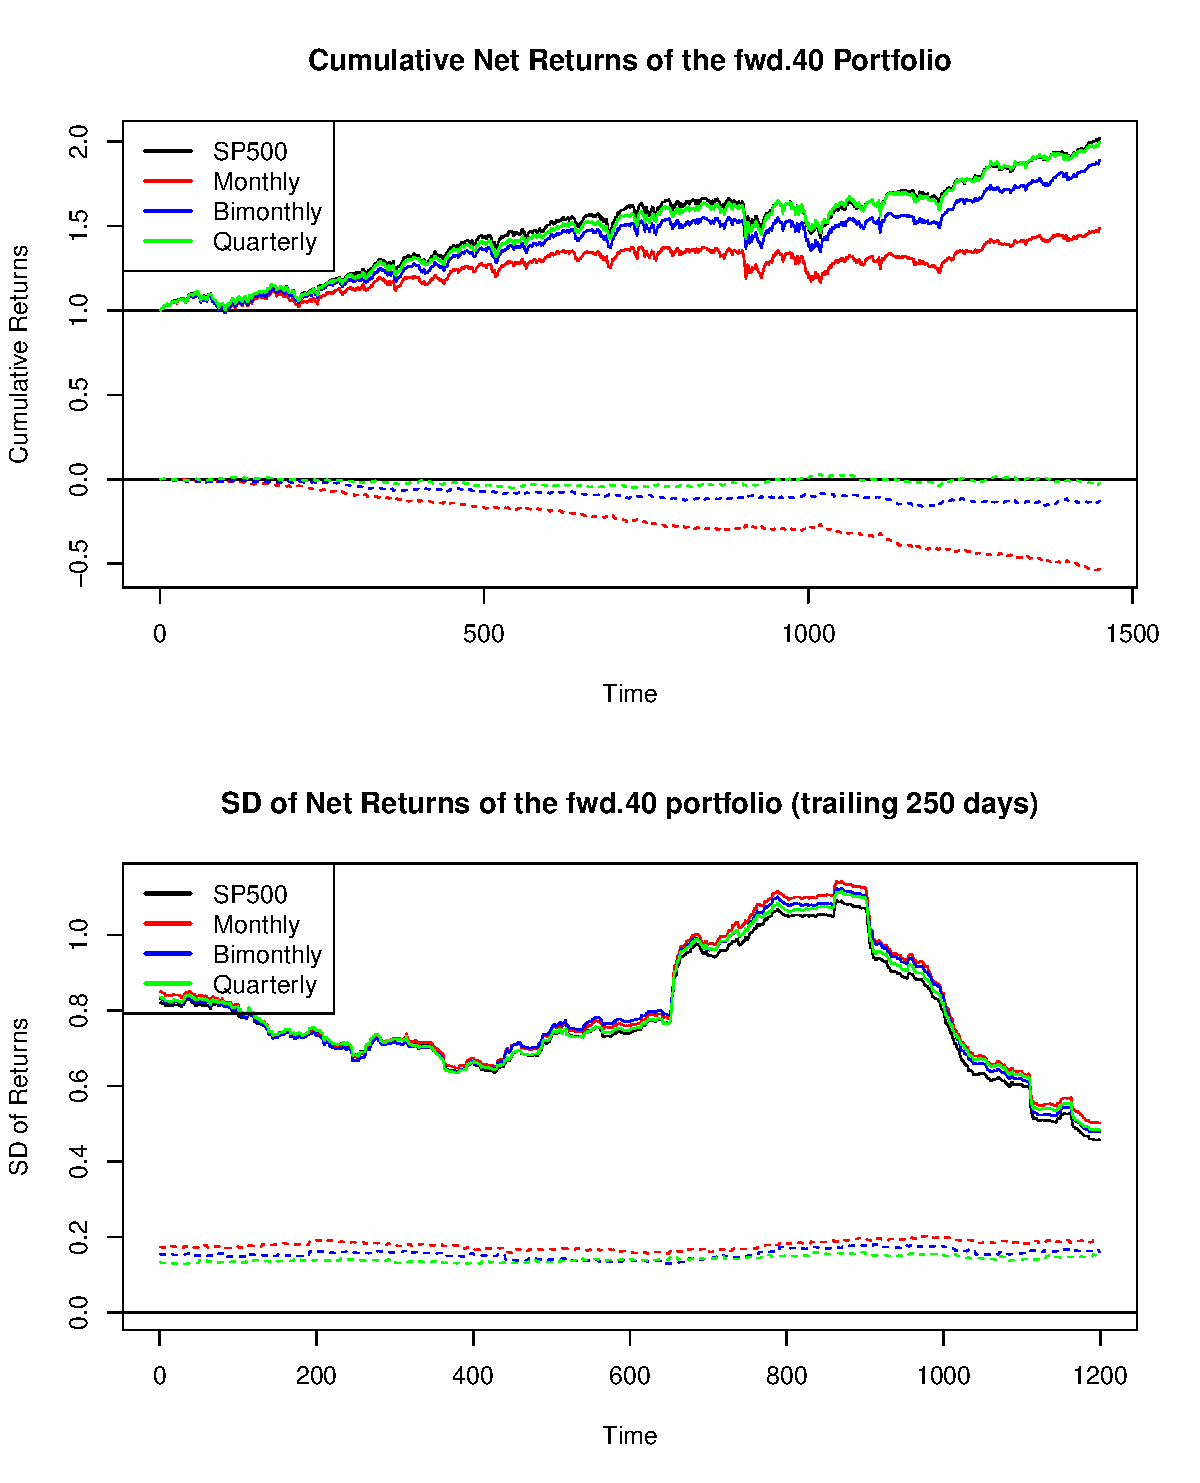
\includegraphics[width=.95\linewidth]{./figs/SP500-retac-fwd-40.pdf}
\begin{quote}
\textbf{Source:} The author.
\end{quote}
\end{figure}

%%%%%%%%%%%%%%%%%%%%%%%%%%%%%%%%%%%%%%%%%%%%%%%%%%%%%%%%%%%%%%%%%%%%%%%%%%%%%%%%%%%%
% SPY LASSO 

\begin{figure}[htpb]
\centering
\footnotesize
\caption{\texttt{las.20} Portfolio (American Data)}
\label{fig:spy:las.20}
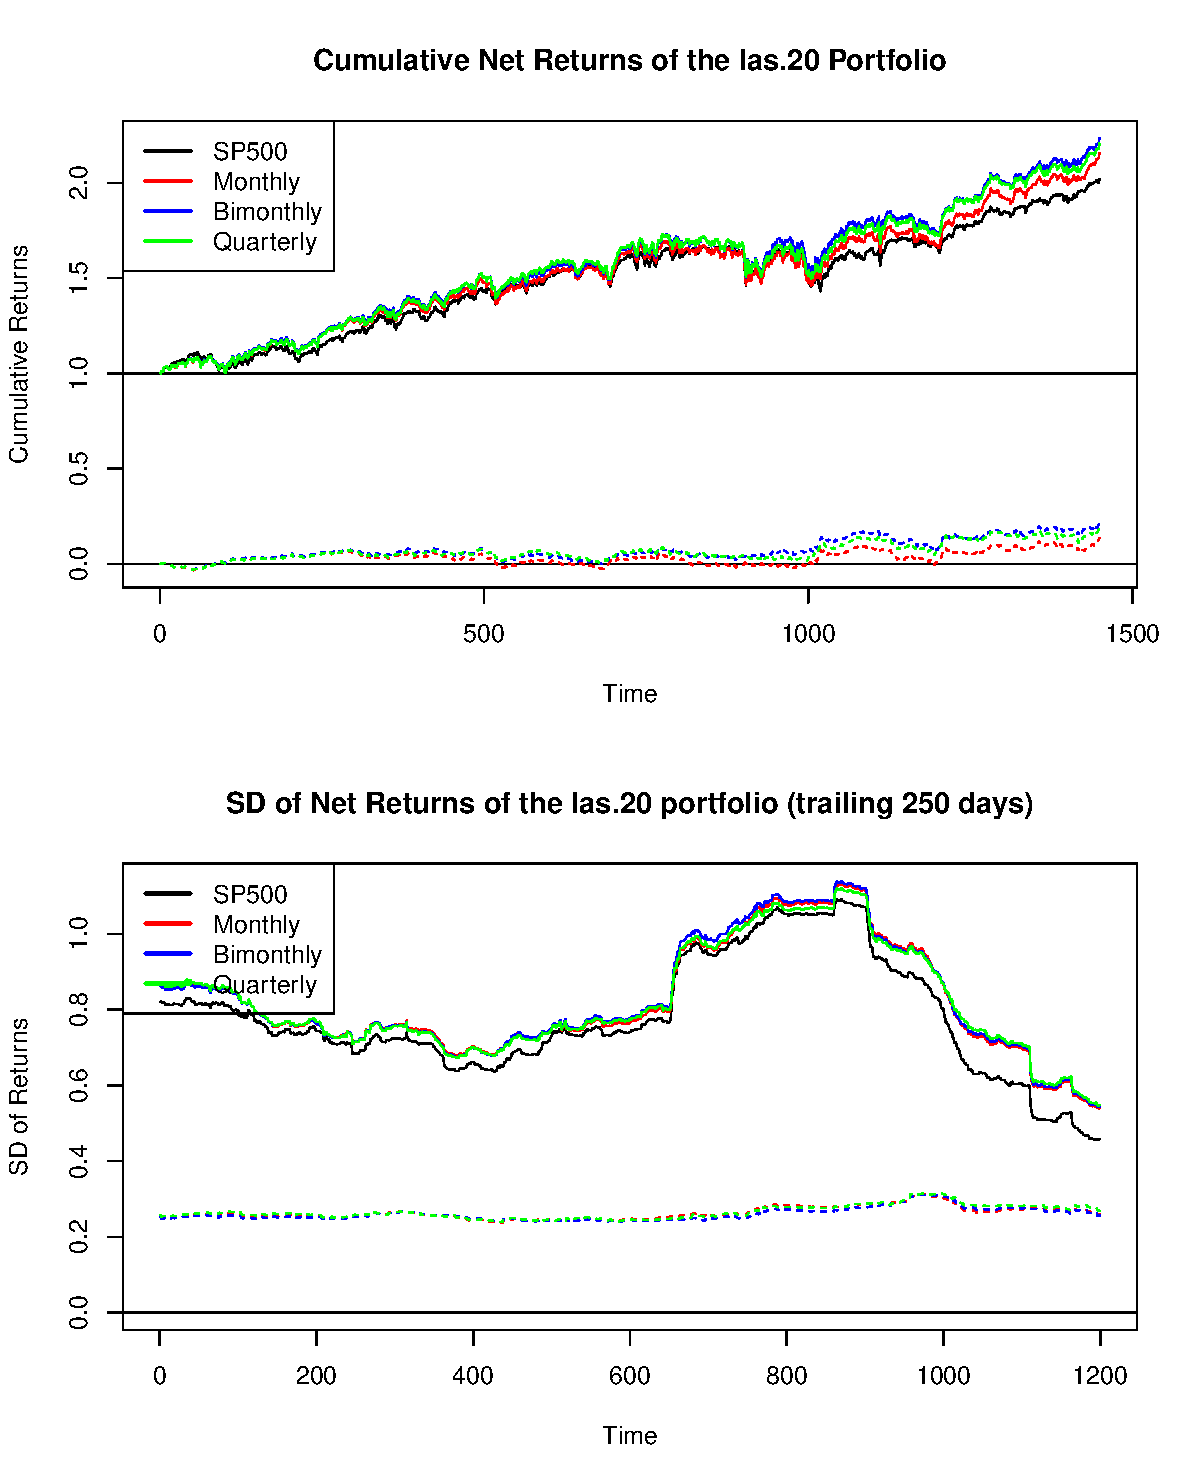
\includegraphics[width=.95\linewidth]{./figs/SP500-retac-las-20.pdf}
\begin{quote}
\textbf{Source:} The author.
\end{quote}
\end{figure}

\begin{figure}[htpb]
\centering
\footnotesize
\caption{\texttt{las.30} Portfolio (American Data)}
\label{fig:spy:las.30}
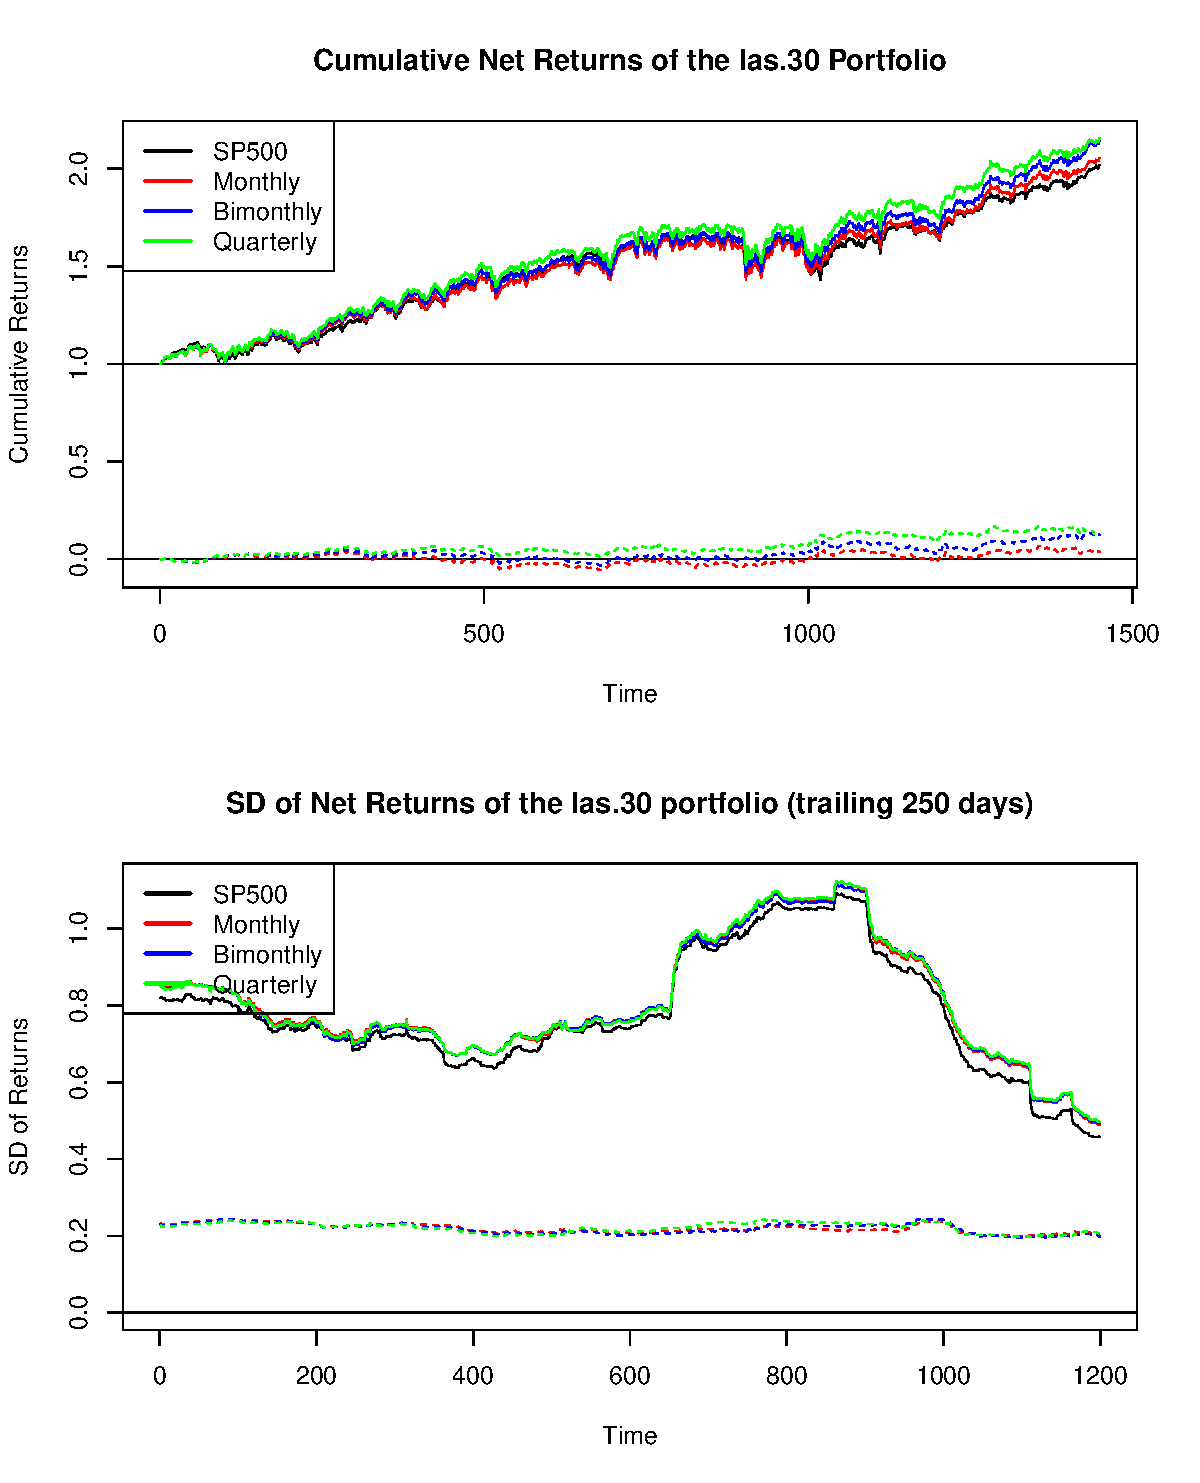
\includegraphics[width=.95\linewidth]{./figs/SP500-retac-las-30.pdf}
\begin{quote}
\textbf{Source:} The author.
\end{quote}
\end{figure}

\begin{figure}[htpb]
\centering
\footnotesize
\caption{\texttt{las.40} Portfolio (American Data)}
\label{fig:spy:las.40}
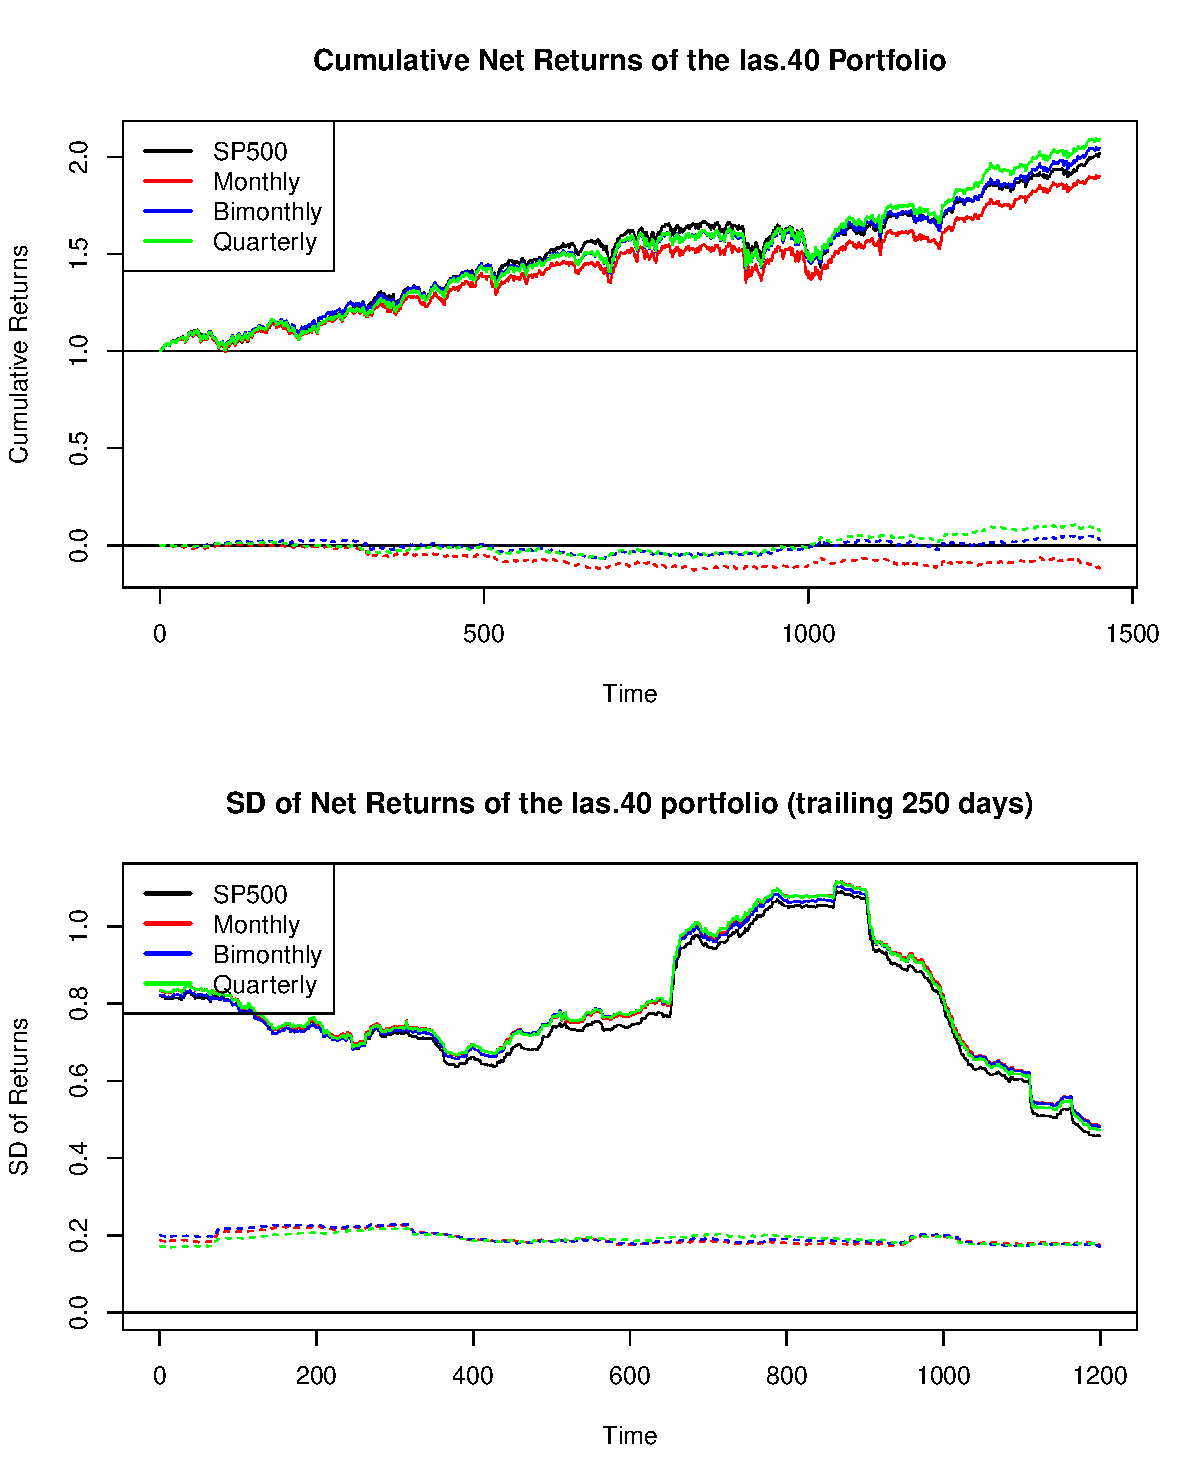
\includegraphics[width=.95\linewidth]{./figs/SP500-retac-las-40.pdf}
\begin{quote}
\textbf{Source:} The author.
\end{quote}
\end{figure}

%%%%%%%%%%%%%%%%%%%%%%%%%%%%%%%%%%%%%%%%%%%%%%%%%%%%%%%%%%%%%%%%%%%%%%%%%%%%%%%%%%%%
% Refrences
\clearpage
\section*{References}
\bibliographystyle{authordate3} % bibliography style
\bibliography{./refs} % References file

%%%%%%%%%%%%%%%%%%%%%%%%%%%%%%%%%%%%%%%%%%%%%%%%%%%%%%%%%%%%%%%%%%%%%%%%%%%%%%%%%%%%
\end{document}

